\documentclass[DynamicalBook]{subfiles}
\begin{document}
%


\setcounter{chapter}{3}%Just finished 3.

\tableofcontents*

%------------ Chapter ------------%
\chapter{Polynomial functors and dynamics}

\slogan{
The category of polynomial functors is a jackpot. Its beauty flows without bound.}

%-------- Section --------%
\section{Introduction}


In this chapter we will investigate a remarkable category called $\poly$. We will see its intimate relationship with both dynamic processes, data storage and transformations, and decision-making. We will see its intimate relationship with safety and decision-making. But our story begins with something quite humble: middle school algebra.
\begin{align}\label{eqn.polynomial1892}
\yon^\2+\yon+\1 \quad&\quad
\textit{polynomial}
\intertext{
All our polynomials will involve one variable, $\yon$, chosen for reasons we'll explain soon. Polynomials in one variable can be depicted as a set of mini-trees:
}
\label{eqn.poly1892}
\begin{tikzpicture}[trees, grow'=up]
  \node (1) {$\bullet$} 
    child {}
    child {};
  \node[right=.5 of 1] (2) {$\bullet$} 
    child {};
  \node[right=.5 of 2] (3) {$\bullet$};
\end{tikzpicture}
\quad&\quad\textit{poly}
\end{align}
More technically, mini-trees are called \emph{corollas}, so what we're calling a \emph{poly} is a set of corollas. 

Intuitively, one might think of each corolla as representing a \emph{decision}. Associated to every decision is a set of \emph{options}. The three decisions we exhibit in \cref{eqn.poly1892} are particularly interesting; they respectively have two options, one option, and no options. Having two options is familiar from life---it's the classic yes/no decision---as well as from Claude Shannon's Information Theory. Having one option is also familiar theoretically and in life: ``sorry, ya just gotta go through it.'' Having no options is when you actually don't get through it: it's ``the end''. While the corollas $\1,\yon,$ and $\yon^\2$ are each interesting as decisions, their sum $\yon^\2+\yon+\1$ has very little theoretical interest; it's just a first example.

In a polynomial like $\4\2\yon^\3+\1\7\yon$, the pure power term $\yon^\3$ has a coefficient of \4\2 next to it, so the corolla with three leaves shows up 42 times%
\footnote{
In standard font, 42 represents the usual natural number. In sans serif font \4\2 represents the set $\4\2=\{1,2,\ldots,42\}$ with 42 elements.
}
in the associated poly. Intuitively, there are 42 situations in which you have a decision with three options. When you put all those decisions together, you have the \emph{arena} associated to $p$. 

Here is a table of terminology. The first column is book-wide terminology, the second is algebraic terminology about polynomials as in \eqref{eqn.polynomial1892}, the third is about the pictures of corollas as in \eqref{eqn.poly1892}, and the fourth column is intuitive terminology.

\begin{equation}\label{eqn.table_terminology}
\small
\begin{tabular}{llll}
\multicolumn{4}{c}{\normalsize Terminology}\\
\textbf{Interface} & \textbf{Polynomial} $p$ & \textbf{Poly} & \textbf{Wheelhouse}\\\hline
Set of positions & $p(\1)$ & Set of roots & Set of situations\\
Interface in position $\fun{i}$ & Pure power summand $\yon^{p_\fun{i}}$ & Corolla & Decision\\
Distinction $c\in p_\fun{i}$ & Element of $p_\fun{i}$ & Leaf & Possibility
\end{tabular}
\end{equation}

If you're wondering about the upright $\fun{i}$, we'll get to all our notational conventions in \cref{sec.poly}.

\begin{exercise}
Consider the polynomial $p\coloneqq\2\yon^\3+\2\yon+\1$ and the associated poly.
\begin{enumerate}
	\item Draw the poly whose name is $p$.
	\item How many roots does this poly have?
	\item How many decisions does this represent?
	\item For each corolla in the poly, say how many leaves it has.
	\item For each decision, how many options does it have?
\end{enumerate}
Now referring instead to the polynomial $q\coloneqq\yon^\nn+\4\yon$:
\begin{enumerate}[resume]
	\item Does the polynomial $q$ have a pure-power summand $\yon^\2$?
	\item Does the polynomial $q$ have a pure-power summand $\yon$?
	\item Does the polynomial $q$ have a pure-power summand $\4\yon$?
	\qedhere
\end{enumerate}

\end{exercise}

Mathematically and notationally we do not make a distinction between a poly and its name $p$; they are two different syntaxes for the same object. 


\begin{exercise}
If you were a suitor choosing the poly you love, aesthetically speaking, which would strike your interest? Answer by circling the associated polynomial:
\begin{enumerate}
	\item $\yon^\2+\yon+\1$
	\item $\yon^\2+\3\yon^\2+\3\yon+\1$
	\item $\yon^\2$
	\item $\yon+\1$
	\item $(\nn\yon)^\nn$
	\item $S\yon^S$
	\item $\yon^{\1\0\0}+\yon^\2+\3\yon$
	\item Your poly's name $p$ here.
\end{enumerate}
Any reason for your choice? Draw a sketch of your poly.
\end{exercise}

Before we can really get into this story, let's summarize where we're going: polynomials are going to have really surprising applications to dynamics, data, and decision. Remember, we spoke superlatively of $\poly$ at the beginning of this chapter,
\slogan{
The category of polynomial functors is a jackpot. Its beauty flows without bound}
and we have not yet begun to deliver. So let's introduce some of the applications and mathematics to come.

%---- Subsection ----%
\subsection{Dynamical systems}

Throughout this book, we've seen dynamical systems---machines of various sorts---which have an internal state that can be read out to other systems, as well as updated based on input received from other systems. In the context of this chapter, we'll be looking mainly at deterministic systems, but with a lot of interesting new options:
\begin{enumerate}
	\item The interface of the system can change shape through time.
	\item The wiring diagram connecting a bunch of systems can change in time.
	\item One can speed up the dynamics of a system.
	\item One can introduce ``effects'', i.e.\ as defined by monads on $\smset$.
	\item The dynamical systems on any interface form a topos.
\end{enumerate}

To give some intuition for the first two, imagine yourself as a system, wired up to other systems. You have some input ports: your eyes, your ears, etc., and you have some output ports: your speech, your gestures, etc. And you connect with other systems: your family, your colleagues, the GPS of your phone, etc.
\begin{equation}\label{eqn.wired_forever}
\begin{tikzpicture}[oriented WD, bb min width =.5cm, bbx=.5cm, bb port sep =1,bb port length=0, bby=.15cm]
	\node[bb={2}{2}, green!25!black] (X11) {\tiny Alice};
	\node[bb={3}{3}, green!25!black, below right=of X11] (X12) {\tiny you};
	\node[bb={2}{1}, green!25!black, above right=of X12] (X13) {\tiny Bob};
	\node[bb={2}{2}, green!25!black, below right = -1 and 1.5 of X12] (X21) {\tiny GPS};
	\node[bb={1}{2}, green!25!black, above right=-1 and 1 of X21] (X22) {\tiny me};
  \node[bb={2}{2}, fit = {($(X11.north east)+(-1,4)$) (X12) (X13) ($(X21.south)$) ($(X22.east)+(.5,0)$)}, bb name = {\small Wired together like this forever?}] (Z) {};
	\draw (X21_out1) to (X22_in1);
	\draw let \p1=(X22.north east), \p2=(X21.north west), \n1={\y1+\bby}, \n2=\bbportlen in
          (X22_out1) to[in=0] (\x1+\n2,\n1) -- (\x2-\n2,\n1) to[out=180] (X21_in1);
	\draw (X11_out1) to (X13_in1);
	\draw (X11_out2) to (X12_in1);
	\draw (X12_out1) to (X13_in2);
	\draw (Z_in1'|-X11_in2) to (X11_in2);	
	\draw (Z_in2'|-X12_in2) to (X12_in2);
	\draw (X12_out2) to (X21_in2);
	\draw (X21_out2) to (Z_out2'|-X21_out2);
	 \draw let \p1=(X12.south east), \p2=(X12.south west), \n1={\y1-\bby}, \n2=\bbportlen in
	  (X12_out3) to[in=0] (\x1+\n2,\n1) -- (\x2-\n2,\n1) to[out=180] (X12_in3);
	\draw let \p1=(X22.north east), \p2=(X11.north west), \n1={\y2+\bby}, \n2=\bbportlen in
          (X22_out2) to[in=0] (\x1+\n2,\n1) -- (\x2-\n2,\n1) to[out=180] (X11_in1);
	\draw (X13_out1) to (Z_out1'|-X13_out1);
\end{tikzpicture}
\end{equation}
We wrote a little question for you at the top of the diagram. Isn't there something a little funny about wiring diagrams? Maybe for old-fashioned machines, you would wire things together once and they'd stay like that for the life of the machine. But my phone connects to different wifi stations at different times, I drop my connection to Alice for weeks at a time, etc. So wiring diagrams should be able to change in time; $\poly$ will let us do that.

\begin{example}
Here are some familiar circumstances where we see wiring diagrams changing in time.
\begin{enumerate}[itemsep=0pt]
%	\item Airplanes only communicate when they get near enough;
%	\item A phone is connected to 4G or to wifi depending on circumstances;
%	\item A person can choose when to open (receive input through) their eyes and when to speak (produce output);\goodbreak
	\item When too much force is applied to a material, bonds can break;
\end{enumerate}
\[
\begin{tikzpicture}[oriented WD, bb small, bb port length=0]
	\foreach \i in {0,...,4} {
		\node[bb={1}{1}, fill=blue!10] at (1.7*\i,0) (X\i) {};
	}
%	\node[bb={1}{1}, fit=(X0) (X4)] (X) {};
	\foreach \i in {0,...,3} {
		\draw[thick] (X\i_out1) -- (X\the\numexpr\i+1\relax_in1);
	};
	\draw[thick, ->] (X0_in1) -- node[above, font=\tiny] {Force} +(-2.5,0);
	\draw[thick, ->] (X4_out1) -- node[above, font=\tiny] {Force} +(2.5,0) node (R) {};
%
\def\x{21};
	\foreach \i in {0,...,2} {
		\node[bb={1}{1}, fill=blue!10] at (\x+1.7*\i,0) (Y\i) {};
	}
	\foreach \i in {3,...,4} {
		\node[bb={1}{1}, fill=blue!10] at (\x+1.3+1.7*\i,0) (Y\i) {};
	}
%	\node[bb={1}{1}, fit=(Y0) (Y4)] (Y) {};
	\foreach \i in {0,1,3} {
		\draw[thick] (Y\i_out1) -- (Y\the\numexpr\i+1\relax_in1);
	};
	\draw[thick, ->] (Y0_in1) -- node[above, font=\tiny] {Force} +(-2.5,0) node (L) {};
	\draw[thick, ->] (Y4_out1) -- node[above, font=\tiny] {Force} +(2.5,0);
	\node[starburst, draw, minimum width=2cm, minimum height=1.5cm,red,fill=orange,line width=1.5pt] at ($(L)!.5!(R)$)
{Snap!};
\end{tikzpicture}
\]
\begin{quote}
In materials science the Young's modulus accounts for how much force can be transferred across a material as its endpoints are pulled apart. When the material breaks, the two sides can no longer feel evidence of each other. Thinking of pulling as sending a signal (a signal of force), we might say that the ability of internal entities to send signals to each other---the connectivity of the wiring diagram---is being measured by Young's modulus. It will also be visible within $\poly$.
\end{quote}
\begin{enumerate}[resume]
	\item A company may change its supplier at any time;
\end{enumerate}
\begin{equation*}%\label{eqn.supplier}
\begin{tikzpicture}[oriented WD, font=\ttfamily, every node/.style={fill=blue!10}, baseline=(c)]
	\node[bb={0}{1}] (s1) {Supplier 1};
	\node[bb={0}{1}, below=of s1] (s2) {Supplier 2};
	\coordinate (helper) at ($(s1)!.5!(s2)$);
	\node[bb={1}{0}, right=1.5 of helper] (c) {Company};
	\draw (s1_out1) to (c_in1);
	\draw (s2_out1) to +(5pt,0) node[fill=none] {$\bullet$};
\begin{scope}[xshift=3.5in]
	\node[bb={0}{1}] (s1') {Supplier 1};
	\node[bb={0}{1}, below=of s1'] (s2') {Supplier 2};
	\coordinate (helper') at ($(s1')!.5!(s2')$);
	\node[bb={1}{0}, right=1.5 of helper'] (c') {Company};
	\draw (s2'_out1) to (c'_in1);
	\draw (s1'_out1) to +(5pt,0) node[fill=none] {$\bullet$};
\end{scope}
	\node[starburst, draw, minimum width=2cm, minimum height=2cm,align=center,fill=green!10, font=\small, fill=white, line width=1.5pt] at ($(c)!.5!(helper')$)
{Change\\supplier!};
\end{tikzpicture}
\end{equation*}
\begin{quote}
The company can get widgets either from supplier 1 or supplier 2; we could imagine this choice is completely up to the company. The company can decide based on the quality of widgets it has received in the past, i.e.\ when the company gets a bad widget, it updates an internal variable, and sometimes that variable passes a threshold making the company switch states. Whatever its strategy for deciding, we should be able to encode it in $\poly$.
\end{quote}
\begin{enumerate}[resume]
	\item When someone assembles a machine, their own outputs dictate the connection pattern of the machine's components.
\end{enumerate}
\begin{equation*}%\label{eqn.someone}
\begin{tikzpicture}[oriented WD, font=\ttfamily, bb port length=0, every node/.style={fill=blue!10}, baseline=(someone.north)]
	\node[bb port sep=.5, bb={0}{1}] (A) {unit A};
	\node[bb port sep=.5, bb={1}{0}, right=of A] (B) {unit B};
	\coordinate (helper) at ($(A)!.5!(B)$);
	\node[bb={1}{1}, below=2 of helper] (someone) {\tikzsymStrichmaxerl[3]};
	\draw[->, dashed, blue] (someone_in1) to[out=180, in=270] (A.270);
	\draw[->, dashed, blue] (someone_out1) to[out=0, in=270] (B.270);
	\draw (A_out1) -- +(10pt,0);
	\draw (B_in1) -- +(-10pt,0);
%
\begin{scope}[xshift=3.5in]
	\node[bb port sep=.5, bb={0}{1}] (A') {unit A};
	\node[bb port sep=.5, bb={1}{0}, right=.5of A'] (B') {unit B};
	\coordinate (helper') at ($(A')!.5!(B')$);
	\node[bb={1}{1}, below=2 of helper'] (someone') {\tikzsymStrichmaxerl[3]};
	\draw[->, dashed, blue] (someone'_in1) to[out=180, in=270] (A'.270);
	\draw[->, dashed, blue] (someone'_out1) to[out=0, in=270] (B'.270);
	\draw (A'_out1) -- (B'_in1);
\end{scope}
%
	\node[starburst, draw, minimum width=2cm, minimum height=2cm,fill=blue!50,line width=1.5pt, align=center, font=\upshape] at ($(B)!.5!(A')-(0,.6cm)$)
{Attach!};
\end{tikzpicture}
\end{equation*}
\begin{quote}
Have you ever assembled something? Your internal states dictate the connection pattern of some other things. We can say this in $\poly$.
\end{quote}

All of the examples discussed here will be presented in some detail once we have the requisite mathematical theory \cref{?,?,?}.
\end{example}

\begin{exercise}
Think of another example where systems are sending each other information, but where the sort of information or who it's being sent to or received from can change based on the states of the systems involved. You might have more than two, say $\rr$-many, different wiring patterns in your situation.
\end{exercise}

But there's more that's intuitively wrong or limiting about the picture in \eqref{eqn.wired_forever}. Ever notice how you can change how you interface with the world? Sometimes I close my eyes, which makes that particular way of sending me information inaccessible: that port vanishes and you need to use your words. Sometimes I'm in a tunnel and my phone can't receive GPS. Sometimes I extend my hand to give or receive an object from another person, but sometimes I don't. My ports themselves change in time. Sometimes I even use my output ports to determine the wiring pattern of other machines. We will be able to say all this using $\poly$.

And there's even more that's wrong with the above description. Namely, when I move my eyes, that's actually something you can see---e.g.\ whether I'm looking at you. When I turn around, I see different things, and \emph{you can notice I'm turned around}! When I use my muscles or mouth to express things, my very position changes: my tongue moves, my body moves. So my output is actually achieved by changing position. The model in $\poly$ will be able to express this too.

\begin{example}
Imagine a million little eyeballs, each of which has a tiny brain inside it, all together in a pond of eyeballs. All that an individual eyeball $e$ can do is open and close. When $e$ is open, it can make some distinction about all the rest of the eyeballs in view: maybe it can count how many are open, or maybe it can see whether just one certain eyeball $e'$ is open or closed. But when $e$ is closed, it can't see anything; whatever else is happening, it's all the same to $e$. All it can do in that state is process previous information.

Each eyeball in this system will correspond to the polynomial $\yon^\ord{n}+\yon$, which intuitively consists of two situations, one with $n$-many options, and the other with only one option.

The point is, however, is that the other eyeballs can tell if $e$ is opened or closed. We can imagine some interesting dynamics in this system, e.g.\ waves of openings or closings sweeping over the group, a ripple of openings expanding through the pond.

Talk about real-world applications!
\end{example}

Hopefully you now have an idea of what we mean by mode-dependence: interfaces and wiring diagrams changing in time, based on the states of all the systems involved. We'll see that $\poly$ speaks about mode-dependent systems and wiring diagrams in this sense. 

But $\poly$ is very versatile in its applications. Next we'll show how it relates to information storage and translation.

%---- Subsection ----%
\subsection{Data}

Data is information, maybe thought of as quantized into atomic pieces, but where these atomic pieces are somehow linked together according to a conceptual structure. When a person or organization uses certain data repeatedly, they often find it useful to put their data in a database. This requires organizing the little pieces into a conceptual structure. So when you hear ``database'', just think of it as a conceptual structure filled with examples.

To fix a mental image, let's say that you need to constantly look up employees, what department they're in, who the admin person is for that department, who their manager is, etc. Here's an associated database
\begin{equation}\label{eqn.mytables}
\begin{tabular}{ c | c  c  c}
  \textbf{Employee}&\textbf{FirstName}&\textbf{WorksIn}&\textbf{Mngr}\\\hline
  1&Alan&101&2\\
  2&Ruth&101&2\\
  3&Carla&102&3
\end{tabular}
\hspace{.3in}
\begin{tabular}{ c | c  c}
  \textbf{Department}&\textbf{Name}&\textbf{Admin}\\\hline
  101&Sales&1\\
  102&IT&3\\~
\end{tabular}
%\hspace{.3in}
%\begin{tabular}{ c |}
%	\textbf{String}\\\hline
%	Alan\\
%	IT\\[-3pt]
%	\resizebox{!}{10pt}{$\vdots$}
%\end{tabular}
\end{equation}
We can see it as being associated to the following conceptual scheme, also called a \emph{schema}:
\begin{equation}\label{eqn.myschema}
\tiny\cat{C}\coloneqq
\boxCD{
\begin{tikzcd}[row sep=large, ampersand replacement = \&]
 	\LTO{Employee}\ar[rr, shift left, "\text{WorksIn}"]\ar[dr, bend right, "\text{FirstName}"']\ar[loop left, "\text{Mngr}"]\&\&
  \LTO{Department}\ar[ll, shift left, "\text{Admin}"]\ar[dl, bend left, "\text{Name}"]\\
  \&\LTO[\circ]{String}
\end{tikzcd}
\\~\\\tiny
  Department.Admin.WorksIn = Department
}
\end{equation}
The equation at the bottom says that for any department $d$, if you ask for the admin person and see which department they work in, it's required to be $d$.

What's called $\cat{C}$ in \eqref{eqn.myschema} is a \emph{finitely presented category}, and the database instance presented in \eqref{eqn.mytables} correspond to a functor $I\colon\cat{C}\to\smset$; it sends the object $\text{Employee}\in\cat{C}$ to the set $I(\text{Employee})\coloneqq\{1,2,3\}$. It sends the morphism $\text{Mngr}\colon\text{Employee}\to\text{Employee}$ to the function $I(\text{Mngr})\colon\{1,2,3\}\to\{1,2,3\}$ given by $I(1)=2$, $I(2)=2$, and $I(3)=3$. A functor $\cat{C}\to\smset$ is called a \emph{copresheaf on $\cat{C}$}. So the story of database schemas and their data can be based on the story of categories and their copresheaves.

There's a very important thing that we do with databases: we query them. We ask them questions like ``tell me everyone that's either the admin person of the Math department or their manager''.
\begin{minted}{mysql}
 FOR    d: Department, e: Employee
 WHERE  Name(d)="Math" AND
        (e=Admin(d) OR e=Mngr(Admin(d)))
 RETURN FirstName(e)
\end{minted}
This sort of question is formally called a ``union of conjunctive queries''. We will see this sort of query is intimately connected with $\poly$.

We will also see how databases can be conceived in terms of dynamical systems.

%---- Subsection ----%
\subsection{Decisions}

Consider the following three trees, the first two are infinite (though that's hard to draw):
\[
\begin{tikzpicture}[trees]
\begin{scope}[
  level 1/.style={sibling distance=20mm},
  level 2/.style={sibling distance=10mm},
  level 3/.style={sibling distance=5mm},
  level 4/.style={sibling distance=2.5mm}]
  \node[dgreen] (a) {$\bullet$}
    child {node[dgreen] {$\bullet$}
    	child {node[dgreen] {$\bullet$}
    		child {node[dgreen] {$\bullet$}
  				child 
  				child
  			}
    		child {node[dyellow] {$\bullet$}
  				child 
  				child
  			}
    	}
    	child {node[dyellow] {$\bullet$}
    		child {node[dgreen] {$\bullet$}
  				child
  				child
  			}
    		child  {node[red] {$\bullet$}}
    	}
    }
    child {node[dyellow] {$\bullet$}
    	child {node[dgreen] {$\bullet$}
    		child {node[dgreen] {$\bullet$}
  				child
  				child
  			}
    		child {node[dyellow] {$\bullet$}
  				child
  				child
  			}
  		}
  		child {node[red] {$\bullet$}
  		}
  	}
  ;
\end{scope}
\begin{scope}[
  level 1/.style={sibling distance=13mm},
  level 2/.style={sibling distance=10mm},
  level 3/.style={sibling distance=5mm},
  level 4/.style={sibling distance=2.5mm}]
\node (b) [right=4 of a, dyellow] {$\bullet$}
  child {node[dgreen] {$\bullet$}
  	child {node[dgreen] {$\bullet$}
  		child {node[dgreen] {$\bullet$}
				child
				child
			}
  		child {node[dyellow] {$\bullet$}
				child
				child
			}
		}
  	child {node[dyellow] {$\bullet$}
  		child {node[dgreen] {$\bullet$}
				child
				child
			}
  		child  {node[red] {$\bullet$}}
  	}
	}
	child {node[red] {$\bullet$}}	
;
\end{scope}
\node (c) [red, right=2 of b] {$\bullet$};
\end{tikzpicture}
\]
These are patterned examples---and we'll understand what this pattern is more clearly in \cref{???}---of what we will call \emph{decision streams}. Decision streams form the objects in a category that also includes the following level-3 abbreviations of binary decision streams (the third of which is a finite stream):
\[
\begin{tikzpicture}[trees]
\begin{scope}[
  level 1/.style={sibling distance=20mm},
  level 2/.style={sibling distance=10mm},
  level 3/.style={sibling distance=5mm},
  level 4/.style={sibling distance=2.5mm}]
  \node (a) {$\bullet$}
    child {node {$\bullet$}
    	child {node {$\bullet$}
    		child {node {$\bullet$}
  			}
    		child {node {$\bullet$}
  				child 
  				child
  			}
    	}
    	child {node {$\bullet$}
  			}
    }
    child {node {$\bullet$}
    	child {node {$\bullet$}
    		child {node {$\bullet$}
  				child
  				child
  			}
    		child {node {$\bullet$}
  				child
  				child
  			}
  		}
  		child {node {$\bullet$}
    		child {node {$\bullet$}
  			}
    		child {node {$\bullet$}
  			}
  		}
  	}
  ;
\end{scope}
\begin{scope}[
  level 1/.style={sibling distance=13mm},
  level 2/.style={sibling distance=10mm},
  level 3/.style={sibling distance=5mm},
  level 4/.style={sibling distance=2.5mm}]
  \node (b) [right=4 of a] {$\bullet$}
    child {node {$\bullet$}
    }
    child {node {$\bullet$}
    	child {node {$\bullet$}
    		child {node {$\bullet$}
  			}
    		child {node {$\bullet$}
  				child
  				child
  			}
  		}
  		child {node {$\bullet$}
    		child {node {$\bullet$}
  				child
  				child
  			}
    		child {node {$\bullet$}
  				child
  				child
  			}
  		}
  	}
  ;
\end{scope}
\begin{scope}[
  level 1/.style={sibling distance=13mm},
  level 2/.style={sibling distance=8mm},
  level 3/.style={sibling distance=5mm},
  level 4/.style={sibling distance=2.5mm}]
  \node (c) [right=4 of b] {$\bullet$}
    child {node {$\bullet$}
    	child {node {$\bullet$}
  		}
  		child {node {$\bullet$}
    		child {node {$\bullet$}
  			}
    		child {node {$\bullet$}
  			}
  		}
    }
    child {node {$\bullet$}
  	}
  ;
\end{scope}
\end{tikzpicture}
\]

The set of such decision streams in fact form the objects of a category with very nice properties (it's a topos), which we call $\sys(\yon^\2+\1)$. The idea is that every corolla in these diagrams has either two options, corresponding to $\yon^\2$, or no options, corresponding to $\1=\yon^\0$.

\begin{exercise}
\begin{enumerate}
	\item Draw a level-3 abbreviation of a decision stream of type $\yon^\2+\yon^\0$.
	\item Draw a level-4 abbreviation of a decision stream of type $\yon$.
	\item Draw a level-3 abbreviation of a decision stream of type $\nn\yon^\2$ by labeling every node with a natural number.
	\qedhere
\end{enumerate}
\end{exercise}

But decisions aren't just about choosing; they're also about trying to accomplish something. The logic of accomplishment is exceptionally rich in this setting. We will concentrate on what we call a \emph{win condition}, which is a subgraph of the decision stream with the property that if $n$ is winning node, then any child of $n$ is also a winning node. 
\[\begin{tikzpicture}[trees,
  level 1/.style={sibling distance=20mm},
  level 2/.style={sibling distance=10mm},
  level 3/.style={sibling distance=5mm},
  level 4/.style={sibling distance=2.5mm}]
  \node (root) {$\bullet$}
    child {node {$\bullet$}
    	child {node {$\bullet$}
    		child {node {$\bullet$}
  			}
    		child {node {$\bullet$}
  				child
  				child
  			}
    	}
    	child {node {$\bullet$}
  			}
    }
    child {node {$\bullet$}
    	child {node {$\bullet$}
    		child {node {$\bullet$}
  				child
  				child
  			}
    		child {node {$\bullet$}
  				child
  				child
  			}
  		}
  		child {node {$\bullet$}
    		child {node {$\bullet$}
  				child
  				child
  			}
    		child {node {$\bullet$}
  			}
  		}
  	}
  ;
 \begin{scope}[every node/.style={circle, inner sep=3pt, blue, draw}]
  \node at (root-1-2)     {};
  \node at (root-2-1-1-1) {};
  \node at (root-2-1-1-2) {};
  \node at (root-2-1-2-1) {};
	\node at (root-2-2) 		{};
  \node at (root-2-2-1) 	{};
  \node at (root-2-2-2) 	{};
  \node at (root-2-2-1-1) {};
  \node at (root-2-2-1-2) {};
 \end{scope}
\end{tikzpicture}
\]
More formally, these are called \emph{sieves}; they form the elements of a logical system called a Heyting algebra: you can take any two sieves and form the intersection or union (which correspond to AND and OR), or even things like implication, negation, and existential and universal quantification. This will give us a calculus of win-conditions for any sort $p$ of decision stream.

%---- Subsection ----%
\subsection{Implementation}

Everything we talk about can actually be implemented in a computer without much difficulty, at least if you have access to a language that supports dependent types. We will continue to use Agda.

What we have been calling polynomials---things like $\yon^\2+\2\yon+\1$---are often called \emph{containers} in the computer science literature. A container consists of a type $S$, usually called the type of \emph{shapes}, and a type $P(s)$ for each term $s:S$, called the type of positions in shape $s$. It's mildly unfortunate that the names clash with our own: for us a container-shape is a position and a container-position is a distinction.

Luckily, the agda code is pretty easy to understand.
\begin{agda}
record Wheelhouse : Set where  -- a arena consists of 
   field                       -- two fields
     decn : Set                -- one called decn, a set, and
     posy : pos -> Set         -- one called posy,
                               -- a set that depends on decn
\end{agda}  

%---- Subsection ----%
\subsection{Mathematical theory}\label{subsec.math_theory}

The applications of $\poly$ are quite diverse and interesting, including dynamics, data, and decisions. However it is how the mathematics of $\poly$ supports these applications that is so fantastic. For experts, here are some reasons for the excitement.

\begin{proposition}
$\poly$ is a biCartesian closed category, meaning it has sums, products, and exponential objects. It supports the simply typed lambda calculus.
\end{proposition}

In fact $\poly$ has infinite coproducts, infinite products, and is completely distributive. We'll explain all of this in \cref{??}; for now we continue with the highlights.

\begin{proposition}
Beyond the coCartesian and Cartesian monoidal structures $(\0,+)$ and $(\1,\times)$, the category $\poly$ has two additional monoidal structures, denoted $(\yon,\otimes)$ and $(\yon,\circ)$, which are together duoidal. Moreover $\otimes$ is also a closed monoidal structure and it distributes over $+$.
\end{proposition}

\begin{proposition}
$\poly$ has an adjoint quadruple with $\smset$ and an adjoint pair with $\smset\op$:
\begin{equation*}%\label{eqn.adjoints_galore}
\begin{tikzcd}[column sep=60pt]
  \smset
  	\ar[r, shift left=7pt, "A" description]
		\ar[r, shift left=-21pt, "A\yon"']&
  \poly
  	\ar[l, shift right=21pt, "p(\0)"']
  	\ar[l, shift right=-7pt, "p(\1)" description]
	\ar[l, phantom, "\scriptstyle\Leftarrow"]
	\ar[l, phantom, shift left=14pt, "\scriptstyle\Rightarrow"]
	\ar[l, phantom, shift right=14pt, "\scriptstyle\Rightarrow"]
\end{tikzcd}
\hspace{.6in}
\adjr[50pt]{\smset\op}{\yon^A}{\Gamma p}{\poly}.
\end{equation*}
Each functor is labeled by where it sends $p\in\poly$ or $A\in\smset$.
\end{proposition}

There's a lot we're leaving out of this summary, just so we can hit the highlights.

\begin{proposition}
The functor $\poly\to\smset$ given by $p\mapsto p(\1)$ is a monoidal fibration.
\end{proposition}

In fact it's a monoidal $*$-bifibration in the sense of \cite{shulman2008framed}. But here's where things get really interesting.

\begin{proposition}[Ahman-Uustalu]\label{prop.ahman_uustalu1}
Comonoids in $(\poly,\yon,\circ)$ are categories (up to isomorphism).
\end{proposition}

\begin{proposition}[Niu]
The category $\comon$ has finite coproducts and products, and coproducts in $\comon$ agree with those in $\smcat$.
\end{proposition}

\begin{proposition}
Suppose that the category $\cat{C}$ corresponds under \cref{prop.ahman_uustalu1}, to the comonoid $\com{C}$. Then there is an equivalence of categories
\[
\Cat{Bimod}(\com{C},0)\cong\cat{C}\set
\]
between $(\com{C},0)$-bimodules and $\cat{C}$-copresheaves.
\end{proposition}
We will use the convention that the comonoid $\com{C}$ corresponds to category $\cat{C}$, and similarly for $\com{D}$ and $\cat{D}$, etc. 

\begin{proposition}[Garner]
For any categories $\cat{C}$ and $\cat{D}$, there is an equivalence of categories
\[
\Cat{Bimod}(\com{C},\com{D})\cong\Cat{pra}(\cat{C}\set,\cat{D}\set)
\]
between that of bimodules between comonoids in $\poly$ and parametric right adjoints between copresheaf categories.
\end{proposition}

\begin{proposition}
The functor $\comon\to\poly$ has a right adjoint
\[
\adjr{\poly}{\com{K}_-}{u_-}{\comon},
\]
called the \emph{cofree comonoid} construction. It is lax monoidal with respect to $\otimes$.
\end{proposition}

\begin{proposition}
The category $\comon$ has a third symmetric monoidal structure $(\yon,\otimes)$, and the functor $u_-\colon(\comon,\yon,\otimes)\to(\poly,\yon,\otimes)$ is strong monoidal.
\end{proposition}



\begin{proposition}[Niu]\label{prop.sysp_is_topos}
For any polynomial $p$, the category
\[\sys(p)\cong\com{K}_p\set\]
of dynamical systems on $p$ forms a topos.
\end{proposition}

\begin{proposition}\label{prop.poly_map_pregeo_topos}
A morphism $p\to q$ of polynomials induces a pre-geometric morphism between their respective toposes
\[
\adj{\sys(p)}{}{}{\sys(q)}.
\]
\end{proposition}

If you skipped over any of that---or all of that---it'll be no problem whatsoever! We will get to everything in the current section, \ref{subsec.math_theory}, over the next few chapters. To briefly summarize the results we have just seen, they say in particular that there is a full-fledged logic of dynamical systems inhabiting any interface (\cref{prop.sysp_is_topos}), that these logics can be combined and compared (\cref{prop.poly_map_pregeo_topos}), and that the whole story of dynamics carries a strong connection to database theory. There are many avenues for study, but we need to push forward.

Let's begin.


%-------- Section --------%
\section{Introduction to $\poly$ as a category}\label{sec.poly}


In this section, we will set down the basic category-theoretic story of $\poly$, so that we can have a firm foundation from which to speak about dynamical systems, decisions, and data. We begin with the category $\smset$ of sets and functions, and what is arguably the fundamental theorem of category theory, the Yoneda lemma.

%---- Subsection ----%
\subsection{Representable functors and the Yoneda lemma}

\begin{definition}
Given any set $S$, we denote by $\yon^S\colon\smset\to\smset$ the functor that sends any set $X$ to the set $X^S=\smset(S,X)$, and sends any function $h\colon X\to Y$ to the function $h^S\colon X^S\to Y^S$, the one that sends $g\colon S\to X$ to $g\then h\colon S\to Y$.

We refer to $\yon^S$ as the functor \emph{represented by} $S$.
\end{definition}

The symbol $\yon$ stands for Yoneda, for reasons we will get to in \cref{lemma.yoneda}. For now, here are some pictures for your eyes to gaze at; they are the poly's corresponding to various representables:
\[
\begin{tikzpicture}[trees, grow'=up, sibling distance=2mm]
  \node["$\yon^{\5}$" below] (1) {$\bullet$} 
    child foreach \i in {1,...,5}
    ;
\end{tikzpicture}
\qquad
\begin{tikzpicture}[trees, grow'=up, sibling distance=1mm]
  \node["$\yon^{\1\0}$" below] (1) {$\bullet$} 
    child foreach \i in {1,...,10}
    ;
\end{tikzpicture}
\qquad
\begin{tikzpicture}[trees, grow'=up, sibling distance=0.5mm]
  \node["$\yon^{\2\0}$" below] (1) {$\bullet$} 
    child foreach \i in {1,...,20}
    ;
\end{tikzpicture}
\qquad
\begin{tikzpicture}[trees, grow'=up, sibling distance=0.25mm]
  \node["$\yon^{\4\0}$" below] (1) {$\bullet$} 
    child foreach \i in {1,...,40}
    ;
\end{tikzpicture}
\qquad
\begin{tikzpicture}[trees, grow'=up, sibling distance=0.0625mm]
  \node["$\yon^{[0,1]}$" below] (1) {$\bullet$} 
    child foreach \i in {1,...,160}
    ;
\end{tikzpicture}
\]

\begin{example}
The functor that sends every set $X$ to $X\times X$, and sends $h\colon X\to Y$ to $(h\times h)\colon (X\times X)\to(Y\times Y)$ is representable. 
\end{example}

\begin{exercise}
For each of the following functors $\smset\to\smset$, say if it is representable or not; if it is, say what the representing set is.
\begin{enumerate}
	\item The identity functor $X\mapsto X$.
	\item The constant functor $X\mapsto\2$.
	\item The constant functor $X\mapsto\1$.
	\item The constant functor $X\mapsto\0$.
	\item The functor $X\mapsto X^\nn$.
	\item The functor $X\mapsto 2^X$.
\qedhere
\end{enumerate}
\end{exercise}

\begin{proposition}\label{prop.representable_nt}
For any function $f\colon R\to S$, there is an induced natural transformation $\yon^f\colon\yon^S\to \yon^R$; on any set $X$ the $X$-component $(\yon^f)_X\colon X^S\to X^R$ is given by sending $g\colon S\to X$ to $f\then g\colon R\to X$.
\end{proposition}

\begin{exercise}
Prove that for any function $f\colon R\to S$, what we said was a natural transformation in \cref{prop.representable_nt} really is natural. That is, for any function $h\colon X\to Y$, show that the following diagram commutes:
\[
\begin{tikzcd}
	X^S\ar[r, "h^S"]\ar[d, "X^f"']&
	Y^S\ar[d, "Y^f"]\\
	X^R\ar[r, "h^R"']&
	Y^R\ar[ul, phantom, "?"]
\end{tikzcd}
\qedhere
\]
\end{exercise}

\begin{exercise}
Let $X=\{a,b,c\}$. For each of the following sets $R,S$ and functions $f\colon R\to S$, describe the $X$-component of, i.e.\ the function $X^S\to X^R$ coming from, the natural transformation $\yon^f\colon\yon^S\to\yon^R$.
\begin{enumerate}
	\item $R=\5$, $S=\5$, $f=\id$.
	\item $R=\2$, $S=\1$, $f$ is the unique function.
	\item $R=\1$, $S=\2$, $f(1)=1$.
	\item $R=\1$, $S=\2$, $f(1)=2$.
	\item $R=\0$, $S=\5$, $f$ is the unique function.
	\item $R=\nn$, $S=\nn$, $f(n)=n+1$.
\qedhere
\end{enumerate}
\end{exercise}

\begin{exercise}
Show that the construction in \cref{prop.representable_nt} is functorial
\begin{equation}
\yon^-\colon\smset\op\to\smset^\smset,
\end{equation}
as follows.
\begin{enumerate}
	\item Show that for any set $S$, we have $\yon^{\id_S}\colon\yon^S\to\yon^S$ is the identity.
	\item Show that for any functions $f\colon R\to S$ and $g\colon S\to T$, we have $\yon^g\then\yon^f=\yon^{f\then g}$.
\qedhere
\end{enumerate}
\end{exercise}

\begin{lemma}[Yoneda lemma]\label{lemma.yoneda}
Given a functor $F\colon\smset\to\smset$ and a set $S$, there is an isomorphism
\begin{equation}\label{eqn.yoneda}
F(S)\cong\nat(\yon^S,F)
\end{equation}
where $\nat$ denotes the set of natural transformations. Moreover, \eqref{eqn.yoneda} is natural in both $S$ and $F$.
\end{lemma}
\begin{proof}[Sketch of proof]
For any natural transformation $m\colon\yon^S\to F$, consider the component $m_S\colon S^S\to F(S)$. Applying it to the identity on $S$ as an element of $S^S$, we get an element $m_S(\id_S)\in F(S)$.

For any element $a\in F(S)$, there is a natural transformation $m_a\colon\yon^S\to F$ whose component on $X$ is the function $X^S\to F(X)$ given by sending $g\colon S\to X$ to $F(g)(a)$. In \cref{exc.finish_proof_yoneda} we ask you to show that this is natural in $X$ and that these two constructions are mutually inverse.
\end{proof}

\begin{exercise}\label{exc.finish_proof_yoneda}
Whoever solves this exercise can say they've proved the Yoneda Lemma.
\begin{enumerate}
	\item Show that for any $a\in F(S)$, the maps $X^S\to F(X)$ given as in \cref{lemma.yoneda} are natural in $X$.
	\item Show that the two mappings from \cref{lemma.yoneda} are mutually inverse.
	\item As a corollary of \cref{lemma.yoneda}, show that $\yon^-\colon\smset\op\to\smset^\smset$ is fully faithful, in particular that there is an isomorphism $\nat(\yon^S,\yon^T)\cong S^T$.
\qedhere
\end{enumerate}
\end{exercise}

%---- Subsection ----%
\subsection{Polynomials: sums of representables}

We've seen that for any set $A$, the symbol $\yon^A$ represents a functor $\smset\to\smset$. We will generalize this by adding representable functors together to form polynomials. In some sense the name ``polynomial'' doesn't quite fit, because in algebra polynomials are often taken to be finite sums, whereas we will use sums that may be infinite. However, we are not the first by far to use this term.

So here's the deal. All of our polynomials will be polynomials in one variable, $\yon$; every other letter or number that shows up will represent a set.%
\footnote{For those who clamor for polynomials in many variables, we will see in \cref{??} that the multivariable story falls out of the one-variable story.}
For example, in the following crazy polynomial
\begin{equation}\label{eqn.crazy_poly}
p\coloneqq\rr\yon^\zz+\3\yon^{\3}+A\yon+\sum_{i\in I}Q_i\yon^{R_i+Q_i^2},
\end{equation}
$\rr$ denotes the set of real numbers, $\zz$ denotes the set of integers, $\3$ denotes the set $\{1,2,3\}$, and $A$, $I$, $Q_i$, and $R_i$ denote some arbitrary sets that should have already been defined in order for \eqref{eqn.crazy_poly} to make sense.

The polynomials we already understand at this point are the pure-power polynomials $\yon^A$ for some set $A$; they are representable functors $\yon^A\colon\smset\to\smset.$
So to understand general polynomials like $p$, we just need to understand sums of functors. It will be useful to discuss products of functors at the same time. However, we haven't discussed sums and products of sets yet, so we need to do that first.

\paragraph{Dependent sums and products of sets.}

Let $I$ be a set, and let $X_i$ be a set for each $i\in I$. We denote this \emph{$I$-indexed collection of sets} by $X\colon I\to\smset$ or more classically as $(X_i)_{i\in I}$. Choosing one element from one set in the collection would be denoted $(i,x)$ where $x\in X_i$. Choosing an element from each set in the collection would be denoted $(x_i)_{i\in I}$, where each $x_i\in X_i$.

\begin{definition}[Dependent sums and products of sets]
Let $I$ be a set and $X\colon I\to\smset$ be an $I$-indexed collection of sets. The sum $\sum_{i\in I}X_i$ (respectively, the \emph{product} $\prod_{i\in I}X_i$) of this collection is the set
\[
\sum_{i\in I}X_i=\{(i,x)\mid i\in I\text{ and }x\in X_i\}
\qqand
\prod_{i\in I}X_i=\{(x_i)_{i\in I}\mid x_i\in X_i\}.
\]
\end{definition}

\begin{example}\label{ex.two_sums_and_prods}
If $I=\2=\{1,2\}$ then a collection $X\colon I\to \smset$ is just two sets, say $X_1=\{a,b,c\}$ and $X_2=\{c,d\}$. The sum is the disjoint union
\[\sum_{i\in \2}X_i=X_1+X_2=\{(1,a),(1,b),(1,c),(2,c),(2,d)\}.\]
Its number of elements (cardinality) will always be the sum of the numbers of elements in $X_1$ and $X_2$. Similarly,
\[\prod_{i\in \2}X_i=X_1\times X_2=\{(a,c),(a,d),(b,c),(b,d),(c,c),(c,d)\}.\]
\end{example}


\begin{exercise}\label{exc.on_sums_prods_sets}
Let $I$ be a set and let $X_i=\1$ be a one-element set for each $i\in I$. 
\begin{enumerate}
	\item Show that there is an isomorphism of sets $I\cong\sum_{i\in I}\1$.
	\item Show that there is an isomorphism of sets $\1\cong\prod_{i\in I}\1$.
\end{enumerate}
As a special case, suppose $I\coloneqq\varnothing$ and $X\colon \varnothing\to\smset$ is the unique empty collection of sets.
\begin{enumerate}
	\item Is it true that $X_i=\1$ for each $i\in I$?
	\item Show that there is an isomorphism of sets $\0\cong\sum_{i\in\varnothing}X_i$.
	\item Show that there is an isomorphism of sets $\1\cong\prod_{i\in\varnothing}X_i$.
\qedhere
\end{enumerate}
\end{exercise}

Where are we, and where are we going? We've define dependent sums and products of sets; that's where we are. Our goal is to define polynomial functors, e.g.\ $\yon^\2+\2\yon+\1$, and the maps between them. Since $\yon^2$, $\yon$, and $\1$ are functors, we just need to define sums of functors $\smset\to\smset$. But we might as well define products of functors at the same time, because they'll very much come in handy.

\paragraph{Dependent sums and products of functors $\smset\to\smset$.}

\begin{definition}[Dependent sums and products of functors $\smset\to\smset$]\label{def.sum_prod}
For any two functors $F,G\colon\smset\to\smset$, let
\[
  (F+G)\colon\smset\to\smset
  \qqand
  (F\times G)\colon\smset\to\smset
\]
denote the functors that respectively assign to each $X\in\smset$ the sets
\[
  (F+G)(X)\coloneqq F(X)+G(X)
  \qqand
	(F\times G)(X)\coloneqq F(X)\times G(X).
\]
More generally, for any set $I$ and functors $(F_i)_{i\in I}$, let
\[
\sum_{i\in I}F_i\coloneq\smset\to\smset
\qqand
\prod_{i\in I}F_i\coloneq\smset\to\smset
\]
denote the functors that respectively assign to each $X\in\smset$ the sum and product of sets
\[
	\Big(\sum_{i\in I}F_i\Big)(X)\coloneqq\sum_{i\in I} F_i(X)
	\qqand
	\Big(\prod_{i\in I}F_i\Big)(X)\coloneqq\prod_{i\in I} F_i(X).
\]
We denote by $\0,\1\colon\smset\to\smset$ the constant functors, which respectively assign $\0$ and $\1$ to each $X\in\smset$.
\end{definition}

\begin{proposition}
Referring to the notation in \cref{def.sum_prod}, the functors $\0$ and $\1$ are respectively an initial object and a terminal object in $\smset^\smset$, the operations $+$ and $\times$ are respectively a binary coproduct and a binary product in $\smset^\smset$, and the operations $\sum_{i\in I}$ and $\prod_{i\in I}$ are arbitrary coproducts and products in $\smset^\smset$.
\end{proposition}
\begin{proof}
By \cref{ex.two_sums_and_prods,exc.on_sums_prods_sets}, it suffices to show that $\sum_{i\in I}F_i$ and $\prod_{i\in I}F_i$ are a sum and product in $\smset^\smset$. This itself is a special case of a more general fact, where sums and products are replaced by arbitrary colimits and limits, and where $\smset^\smset$ is replaced by an arbitrary functor category $\cat{C}^\cat{D}$, where $\cat{C}$ is a category that (like $\smset$) has limits and colimits; see \cite[page 22 -- 23, displays (24) and (25)]{macLane1992sheaves}.
\end{proof}

We've finally arrived: we can define the category of polynomial functors!

\paragraph{$\poly$, the category of polynomial functors}

\begin{definition}[Polynomial functors]
A \emph{polynomial functor} is a functor $p\colon\smset\to\smset$ such that there exists a set $I$, sets $(p_i)_{i\in I}$, and an isomorphism
\[p\cong\sum_{i\in I}\yon^{p_i}\]
to a sum of representables.
A \emph{morphism of polynomial functors} is simply a natural transformation $p\to q$.
\end{definition}

So (up to isomorphism), a polynomial functor is just a sum of representables.

\begin{example}\label{ex.pedantic_poly_eval}
Consider the polynomial $\yon^\2+\2\yon+\1$. It denotes a functor $\smset\to\smset$; what does this functor do to the set $X\coloneqq\{a,b\}$? 
To be very precise and pedantic, let's say
\[
I\coloneqq\4\qqand
  p_1\coloneqq\2,\quad
  p_2\coloneqq\1,\quad
  p_3\coloneqq\1,\quad
  p_4\coloneqq\0\
\]
so that $p\cong\sum_{i\in I}\yon^{p_i}$. Now we have
\[
p(X)\cong
\{(1,a,a),(1,a,b),(1,b,a),(1,b,b),(2,a),(2,b),(3,a),(3,b),(4)\}.
\]
It has $(2^2+2+2+1)$-many, i.e.\ $9$, elements. The representable summand $\yon^A$ throws in all $A$-tuples from $X$, but it's indexed by the name of the summand. In particular if $A=\varnothing$ then it just records the empty tuple at that summand.
\end{example}

\begin{exercise}
In the pedantic style of \cref{ex.pedantic_poly_eval}, write out all the elements of $p(X)$ for $p$ and $X$ as follows:
\begin{enumerate}
	\item $p\coloneqq\yon^\3$ and $X\coloneqq\{4,9\}.$
	\item $p\coloneqq\3\yon^\2+\1$ and $X\coloneqq\{a\}$.
	\item $p\coloneqq\0$ and $X\coloneqq\nn$.
	\item $p\coloneqq\4$ and $X\coloneqq\nn$.
	\item $p\coloneqq\yon$ and $X\coloneqq\nn$.
\qedhere
\end{enumerate}
\end{exercise}

\begin{example}
Suppose $p\coloneqq\yon^\2+\2\yon+1$. As a functor $\smset\to\smset$ it should be able to act not only on sets but on functions. Let $X\coloneqq\{a_1,a_2,b_1\}$, $Y\coloneqq\{a,b,c\}$ and $f\colon X\to Y$ the function sending $a_1,a_2\mapsto a$ and $b_1\mapsto b$. The induced function $p(f)\colon p(X)\to p(Y)$ is shown below
\[
\begin{tikzcd}[row sep=2pt, column sep=3pt, shorten <=-5pt, shorten >=-5pt, dashed]
\LMO{(1,a_1,a_1)}\ar[rrrr, blue, bend left=25pt]&\LMO{(1,a_1,a_2)}\ar[rrr, blue, bend left=25pt]&\LMO{(1,a_1,b_1)}\ar[rrr, blue, bend left=25pt]&[30pt]&
\LMO{(1,a,a)}&\LMO{(1,a,b)}&\LMO{(1,a,c)}&&
\\
\LMO{(1,a_2,a_1)}\ar[rrrru, blue, bend left=10pt]&\LMO{(1,a_2,a_2)}\ar[rrru, blue, bend left=10pt]&\LMO{(1,a_2,b_1)}\ar[rrru, blue, bend left=10pt]&&
\LMO{(1,b,a)}&\LMO{(1,b,b)}&\LMO{(1,b,c)}&&
\\
\LMO{(1,b_1,a_1)}\ar[rrrru, blue, bend left=10pt]&\LMO{(1,b_1,a_2)}\ar[rrru, blue, bend left=10pt]&\LMO{(1,b_1,b_1)}\ar[rrru, blue, bend left=10pt]&&
\LMO{(1,c,a)}&\LMO{(1,c,b)}&\LMO{(1,c,c)}&&
\\
\LMO{(2,a_1)}\ar[rrrr, blue, bend left=25pt]&\LMO{(2,a_2)}\ar[rrr, blue, bend left=25pt]&\LMO{(2,b_1)}\ar[rrr, blue, bend left=25pt]&&
\LMO{(2,a)}&\LMO{(2,b)}&\LMO{(2,c)}&&
\\
\LMO{(3,a_1)}\ar[rrrr, blue, bend left=25pt]&\LMO{(3,a_2)}\ar[rrr, blue, bend left=25pt]&\LMO{(3,b_1)}\ar[rrr, blue, bend left=25pt]&&
\LMO{(3,a)}&\LMO{(3,b)}&\LMO{(3,c)}&&
\\&
\LMO{(4)}\ar[rrrr, blue]&&&&\LMO{(4)}
\end{tikzcd}
\]
\end{example}

\begin{exercise}
Let $p=\yon^\2+\yon$. Choose a function $f\colon\1\to\2$ and write out the induced function $p(f)\colon p(\1)\to p(\2)$.
\end{exercise}

\begin{proposition}\label{prop.apply1}
Let $p\coloneqq\sum_{i\in I}\yon^{p_i}$ be an arbitrary polynomial functor. Then $I\cong p(\1)$, so there is an isomorphism of functors
\begin{equation}\label{eqn.sum_p1}
p\cong\sum_{i\in p(\1)}\yon^{p_i}.
\end{equation}
\end{proposition}
\begin{proof}
We need to show that $I\cong p(\1)$; the latter claim follows directly. In \cref{exc.on_sums_prods_sets} it was shown that $I\cong\sum_{i\in I}\1$, so we just need to show that $(\yon^A)(\1)\cong\1$ for any $A\in\smset$. But $1^A\cong 1$ because there is a unique function $A\to 1$ for any $A$.
\end{proof}

The notation in \eqref{eqn.sum_p1} will be how we denote arbitrary polynomials from now on.

\begin{exercise}\label{exc.apply0}
We saw in \cref{prop.apply1} that for any polynomial $p$, e.g.\ $p=\yon^3+3\yon^2+4$, the set $p(\1)$ gives back the set of summands, in this case $\8$. 

What does $p(\0)$ give you?
\end{exercise}

%---- Subsection ----%
\subsection{Understanding morphisms between polynomial functors}
\label{subsec.understanding_mor_poly}

For a seasoned category theorist, we've already said enough to calculate the set $\poly(p,q)$ of morphisms between polynomials $p$ and $q$: it's the set of natural transformations between $p$ and $q$, which are sums of representable functors. But it is worth going over this subject at a more leisurely pace, because it helps us insert some intuition that will be very useful later.

In particular, we're going to think about polynomials like $p$ and $q$ using the intuition from the beginning of the chapter, around the table in \eqref{eqn.table_terminology}. We said that we'd think of $p$ as a arena: a set of decisions you can make and what options you have. That is, $p(\1)$ is conceived as a set of decisions, and for every decision $i\in p(\1)$, we conceive of the set $p_i$ as the options or \emph{options} available in that decision. Here's an alternative way to write $p$:
\[
\begin{tikzcd}
p(\1)\ar[r, "p_-"]&\smset
\end{tikzcd}
\]
Again, every decision $i\in p(\1)$ gets a set $p_i$ of options: that's the whole content of $p$.

The maps $f\colon p\to q$ of polynomials are then the ways to \emph{delegate} $p$'s decisions to $q$. Every one of $p$'s decisions, say $i\in p(\1)$, is passed forward to a decision $j\in q(\1)$ for $q$ to make, and every choice $d\in q_j$ that $q$ could make among its options is passed back as some choice $c\in p_i$ among $p$'s options.

\begin{agda}
record Delegation (w : Wheelhouse) (w' : Wheelhouse) : Set where
   field 
     passfwd : (decn p) -> (decn q)
     passbck : (d : decn p) -> posy q (passfwd d) -> posy p d
\end{agda}

Let's state this mathematically and prove it.

\begin{proposition}\label{prop.poly_maps_colax_prod_sum}
Let $p\coloneqq\sum_{i\in p(\1)}\yon^{p_i}$ and $q\coloneqq\sum_{j\in q(\1)}\yon^{q_j}$ be polynomials. A morphism $p\to q$ can be identified with a pair $(f_1,f^\sharp)$
\begin{equation}\label{eqn.colax_poly_map}
\begin{tikzcd}[column sep=small]
	p(\1)\ar[dr, "p_-"']\ar[rr, "f_1"]&~&
	q(\1)\ar[dl, "q_-"]\\&
	\smset\ar[u, phantom, near end, "\overset{f^\sharp}{\Leftarrow}"]
\end{tikzcd}
\end{equation}
where $f_1$ is a function (or functor between discrete categories) and $f^\sharp$ is a natural transformation: for each $i\in p(\1)$ with $j\coloneqq f_1(i)$, there is a function $f^\sharp_i\colon q_j\to p_i$.

To summarize, we have an isomorphism
\begin{equation}\label{eqn.main_formula}
\poly(p,q)\cong\prod_{i\in p(\1)}\sum_{j\in q(\1)}{p_i}^{q_j}.
\end{equation}
\end{proposition}
\begin{proof}
We have the following isomorphisms
\begin{align*}
  \poly(p,q)&=
  \nat\Big(\sum_{i\in p(\1)}\yon^{p_i},\;\sum_{j\in q(\1)}\yon^{q_j}\Big)&
  	\text{Definitions}\\&\cong
  \prod_{i\in p(\1)}\nat\Big(\yon^{p_i},\sum_{j\in q(\1)}\yon^{q_j}\Big)&
  	\text{Univ. prop. of coproduct}\\&\cong
  \prod_{i\in p(\1)}\sum_{j\in q(\1)}{p_i}^{q_j}&
  	\text{Yoneda lemma}
\end{align*}
This proves what we called the summary. It says that a morphism $p\to q$ consists of: for every $i\in p(\1)$ both a choice of $j\in q(\1)$ and a function from $q_j\to p_i$; the first part determines $f_1$ (i.e.\ $f_1(i)=j$) and the second part just gives $f^\sharp_i$ directly for each $i$.
\end{proof}

The formula in \eqref{eqn.main_formula} will be quite important to us; we will call it our \emph{main formula} for the set of polynomial maps.

\begin{example}\label{ex.practice_with_poly_morphisms}
Let $p\coloneqq \yon^\3+\2\yon$ and $q\coloneqq\yon^\4+\yon^\2+\2$
\[
\begin{tikzpicture}[rounded corners]
	\node (p1) [draw, blue!50!black, "$p$" above] {
	\begin{tikzpicture}[trees, grow'=up, sibling distance=2.5mm]
    \node["\tiny 1" below] (1) {$\bullet$} 
      child {}
      child {}
      child {};
    \node[right=.5 of 1,"\tiny 2" below] (2) {$\bullet$} 
      child {};
    \node[right=.5 of 2,"\tiny 3" below] (3) {$\bullet$}
      child {};
  \end{tikzpicture}
  };
%
	\node (p2) [draw, red!50!black, right=2 of p1, "$q$" above] {
	\begin{tikzpicture}[trees, grow'=up, sibling distance=2.5mm]
    \node["\tiny 1" below] (1) {$\bullet$} 
      child {}
      child {}
      child {}
      child {};
    \node[right=.5 of 1,"\tiny 2" below] (2) {$\bullet$} 
      child {}
      child {};
    \node[right=.5 of 2,"\tiny 3" below] (3) {$\bullet$}
    ;
    \node[right=.5 of 3,"\tiny 4" below] (4) {$\bullet$}
    ;
  \end{tikzpicture}
  };
\end{tikzpicture}
\]
To give a morphism of polynomials $p\to q$, one delegates each $p$-decision $i\in p(\1)$ to a $q$-decision $j\in q(\1)$, and then each option in $q_j$ is passed back to one in $p_i$.

How many ways are there to do this? Before answering this, let's just pick one.
\[
\begin{tikzpicture}
	\node (p1) {
	\begin{tikzpicture}[trees, grow'=up, sibling distance=2.5mm]
    \node[blue!50!black, "\tiny 1" below] (1) {$\bullet$} 
      child {coordinate (11)}
      child {coordinate (12)}
      child {coordinate (13)};
    \node[right=1.5 of 1, red!50!black, "\tiny 1" below] (2) {$\bullet$} 
      child {coordinate (21)}
      child {coordinate (22)}
      child {coordinate (23)}
      child {coordinate (24)};
    \draw[|->, shorten <= 3pt, shorten >= 3pt] (1) -- (2);
    \begin{scope}[densely dotted, bend right]
      \draw (21) to (13);
      \draw (22) to (11);
      \draw (23) to (13);
      \draw (24) to (13);
    \end{scope}
  \end{tikzpicture}	
	};	
%
	\node (p2) [right=1 of p1] {
	\begin{tikzpicture}[trees, grow'=up, sibling distance=2.5mm]
    \node[blue!50!black, "\tiny 2" below] (1) {$\bullet$} 
      child {coordinate (11)};
    \node[right=of 1, red!50!black, "\tiny 1" below] (2) {$\bullet$} 
      child {coordinate (21)}
      child {coordinate (22)}
      child {coordinate (23)}
      child {coordinate (24)};
    \draw[|->, shorten <= 3pt, shorten >= 3pt] (1) -- (2);
    \begin{scope}[densely dotted, bend right]
      \draw (21) to (11);
      \draw (22) to (11);
      \draw (23) to (11);
      \draw (24) to (11);
    \end{scope}
  \end{tikzpicture}	
	};	
%
	\node (p3) [below right=-1.05cm and 1 of p2] {
	\begin{tikzpicture}[trees, grow'=up, sibling distance=2.5mm]
    \node[blue!50!black, "\tiny 3" below] (1) {$\bullet$} 
      child {};
    \node[right=of 1, red!50!black, "\tiny 4" below] (2) {$\bullet$} 
		;
    \draw[|->, shorten <= 3pt, shorten >= 3pt] (1) -- (2);
  \end{tikzpicture}	
	};	
\end{tikzpicture}
\]
This represents one morphism $p\to q$.

So how many different morphisms are there from $p$ to $q$? One way to figure it out is to use the formula \eqref{eqn.main_formula}, but that might need some explaining; we go through such notation in an interlude after \cref{exc.practice_poly_maps}. For now, we can just count ``pre-theoretically''.

The first $p$-decision can be delegated to $q$-decision 1, 2, 3, or 4. Delegating it to the first $q$-decision requires choosing how each of the four options $(q_1=\4)$ are to be assigned one of $p_1=\3$ options; there are $3^4$ ways to do this. Similarly, we can calculate all the ways to delegate the first $p$-decision: there are $3^4+3^2+3^0+3^0=92$. 

The second $p$-decision can be delegated to $q$-decision 1, 2, 3, or 4. There are $1^4+1^2+1^0+1^0=4$ ways to do this; similarly there are four ways to delegate the third $p$-decision to a $q$-decision.

In total, there are $92*4*4=1472$ morphisms $p\to q$, just twenty less than the number of years between Jesus's famous year and Columbus's famous year. Coincidence? 
\end{example}

\begin{exercise}\label{exc.practice_poly_maps}
\begin{enumerate}
	\item Draw the poly's (unions of corollas as in \cref{eqn.poly1892}) associated to $p\coloneqq\yon^3+\yon+1$, $q\coloneqq \yon^2+\yon^2+2$, and $r\coloneqq\yon^3$.
	\item Give an example of a morphism $p\to q$ and draw it as we did in \cref{ex.practice_with_poly_morphisms}.
	\item Explain your morphism as a ``delegation'' in the sense of \cref{subsec.understanding_mor_poly}.
	\item Explain in those terms why there can't be any morphisms $p\to r$.
\qedhere
\end{enumerate}
\end{exercise}

\begin{exercise}
For any polynomial $p$ and set $A$, e.g.\ $A=\2$, the Yoneda lemma gives an isomorphism $p(A)\cong \poly(\yon^A,p)$.
\begin{enumerate}
	\item Choose a polynomial $p$ and draw the associated poly as well as $\yon^\2$.
	\item Count all the maps $\yon^2\to p$.
	\item Is it equal to $p(\2)$?
\qedhere
\end{enumerate}
\end{exercise}

\paragraph{Working with $\sum$ and $\prod$ formulas.}
Here's how to understand and work with a set that involves $\sum$'s and $\prod$'s, e.g.\ something like
\begin{equation}\label{eqn.misc98339}
\sum_{i\in I}\prod_{j\in J(i)}\sum_{k\in K(i,j)}X(i,j,k).
\end{equation}
To understand it, you ask ``what is involved in choosing an element of this set?'' 

The answer given by the formula \eqref{eqn.misc98339} begins by saying ``To choose an element of \eqref{eqn.misc98339}, first..." and then you begin pronouncing the formula. Every time you see $\sum_{i\in I}...$, say ``choose an element $i\in I$; then, ...''. Every time you see $\prod_{j\in J}$, say ``for each $j\in J$, ...''. At the very end when you see some $X$, say ``conclude by choosing an element of $X$''.

So the formula in \eqref{eqn.misc98339} would be pronounced as follows:
\begin{quote}
To choose an element of \eqref{eqn.misc98339}, first choose an element $i\in I$. Then, for every $j\in J(i)$, choose an element $k\in K(i,j)$; then, conclude by choosing an element of $X(i,j,k)$.
\end{quote}
Note that the choice of $k\in k(i,j)$ can depend on $i$ and $j$; it must be able to because these sets $K(i,j)$ can be different for different $i,j$.

\begin{example}[Notation for $\sum\prod$ stuff]\label{ex.notation_sum_prod}
Here we give notation for the elements of a set involving $\sum$'s and $\prod$'s such as that in \eqref{eqn.misc98339}.

Let $I=\{1,2\}$, let $J(1)=\{j\}$ and $J(2)\coloneqq\{j,j'\}$, let $K(1,j)\coloneqq\{k_1,k_2\}$, $K(2,j)\coloneqq\{k_1\}$, and $K(2,j')\coloneqq\{k'\}$, and let $X(i,j,k)=\{x,y\}$ for all $i,j,k$. Now the formula 
\[\sum_{i\in I}\prod_{j\in J(i)}\sum_{k\in K(i,j)}X(i,j,k)\]
 has been given meaning as an actual set. Here is a list of all eight of its elements:
\[
\left\{
\begin{gathered}
	\big(1, j\mapsto(k_1,x)\big),\qquad
	\big(1, j\mapsto(k_1,y)\big),\qquad
	\big(1, j\mapsto(k_2,x)\big),\qquad
	\big(1, j\mapsto(k_2,y)\big),\\
	\big(2, j\mapsto(k_1,x), j'\mapsto(k_1,x)\big),\qquad
	\big(2, j\mapsto(k_1,x), j'\mapsto(k_1,x)\big),\\
	\big(2, j\mapsto(k_1,x), j'\mapsto(k_1,x)\big),\qquad
	\big(2, j\mapsto(k_1,x), j'\mapsto(k_1,x)\big)
\end{gathered}
\right\}
\]
In each case, we first chose an element $i\in I$, either 1 or 2. Then for each $j\in J(i)$ we chose an element $k\in K(i,j)$; then we concluded by choosing an element of $X(i,j,k)$.
\end{example}

\begin{exercise}
With $I$, $J$, $K$, and $X$ as in \cref{ex.notation_sum_prod}, consider the set
\[\prod_{i\in I}\sum_{j\in J(i)}\prod_{k\in K(i,j)}X(i,j,k).\]
\begin{enumerate}
	\item Pronounce it using the ``To choose an element'' formulation just below \eqref{eqn.misc98339}.
	\item How many elements are in it?
	\item Write out three of them in the style of \cref{ex.notation_sum_prod}.
\qedhere
\end{enumerate}
\end{exercise}

The following is sometimes called the \emph{type-theoretic axiom of choice} or the \emph{completely distributive property}, in this case of $\smset$.

\begin{proposition}[Pushing $\prod$ past $\sum$]
For any set $I$, collection of sets $\{J(i)\}_{i\in I}$ and collection of sets $\{X(i,j)\}_{i\in i, j\in J(i)}$, we have a bijection
\begin{equation}\label{eqn.set_completely_distributive}
\prod_{i\in I}\sum_{j\in J(i)}X(i,j)\cong\sum_{j\colon\prod_{i\in I}J(i)}\;\prod_{i\in I}X(i,j).
\end{equation}
\end{proposition}
\begin{proof}
This is almost trivial, once you understand what it's saying; for example once the statement is written, the proof is one line of agda code. An element of the left-hand side is, for each $i\in I$ a choice  of $j_i\in J(i)$ and an element $x_{i,j_i}\in X(i,j_i)$. An element of the right-hand side is a choice of, for each $i\in I$ an element $j(i)\in J(i)$, together with, for each $i$ in $I$ an element $x_{i,j(i)}\in X(i,j(i))$. These are in obvious bijection.
\end{proof}
Below, e.g.\ in \cref{exc.practice_sum_prod}, you'll often see alternating sums and products; using \cref{eqn.set_completely_distributive}, you can always put it into sums-then-products (``disjunctive normal'') form.

When $J(i)=J$ does not depend on $i\in I$, the formula in \eqref{eqn.set_completely_distributive} is much easier:
\[
\prod_{i\in I}\sum_{j\in J}X(i,j)\cong\sum_{j\colon I\to J}\;\prod_{i\in I}X(i,j).
\]

\paragraph{Back to maps of polynomials}
After that interlude, you are hopefully more comfortable with our main formula \cref{eqn.main_formula} describing the set of morphisms between two arbitrary polynomial functors. Let's practice.

\begin{example}[Constants are sent to constants]\label{ex.const_to_const}
Any morphism $p\to q$ must send constants in $p$ to constants in $q$. So if $p$ has constant terms and $q$ doesn't, e.g.\ if $p=\yon^\2+\1$ and $q=\yon^3$, then there are no maps $p\to q$. 

Indeed, let's more generally say $p\coloneqq\sum_{i\in p(\1)}\yon^{p_i}$ and $q\coloneqq\sum_{j\in q(\1)}\yon^{q_j}$ are polynomials, and that we have a map $p\to q$, i.e.\ an element of the set $\prod_{i\in p(\1)}\sum_{j\in q(\1)}{p_i}^{q_j}$. If there is some $i_0\in p(\1)$ such that $p_{i_0}=\0$, then the formula says that for $i_0$ our map has chosen a $j\in q(1)$ and a function $q_j\to p_i$. But in order for such a function to exist, if $p_i$ is empty, $q_j$ must be too.
\end{example}

\begin{exercise}
For each of the following $p,q$, count the number of morphisms $p\to q$:
\begin{enumerate}
	\item $p=\yon^3$,\quad $q=\yon^4$.
	\item $p=\yon^3+1$,\quad $q=\yon^4$.
	\item $p=\yon^3+1$,\quad $q=\yon^4+1$.
	\item $p=4\yon^3+3\yon^2+\yon$,\quad $q=\yon$.
	\item $p=4\yon^3$,\quad $q=3\yon$.
\qedhere
\end{enumerate}
\end{exercise}

%---- Subsection ----%
\subsection{Prepare for dynamics}

As beautiful as the category $\poly$ is---and to be clear we have not really begun to say what is so special about it---discussing its virtues is not our goal. We want to use it!

Polynomial functors are a setting in which to speak about dynamics, data, and decision. We want the reader to understand this deeply as they go through the mathematics. So in order to make the story a bit more seamless, we discuss a few relevant aspects of $\poly$ that we can use immediately.


\paragraph{Finite products}
The category $\poly$ has limits and colimits, is Cartesian closed, has epi-mono factorizations, is completely distributive, etc., etc. However, in order to tell a good story of dynamics, we only need finite products right now. These will be useful for letting many different interfaces control the same internal dynamics.

\begin{proposition}\label{prop.poly_times}
The category $\poly$ has finite products. 
\end{proposition}
\begin{proof}
We will see that $\1$ is a terminal object and that the product of $p$ and $q$ in $\poly$ is the usual product of $p$ and $q$ as polynomials. That is, if $p\coloneqq\sum_{i\in p(\1)}\yon^{p_i}$ and $q\coloneqq\sum_{i\in q(\1)}\yon^{q_i}$ are in standard notation, then
\begin{equation}\label{eqn.poly_times}
p\times q\cong\sum_{i\in p(\1)}\sum_{j\in q(\1)}\yon^{p_i+q_j}.
\end{equation}
We leave the proof as an exercise; see \cref{exc.poly_times}.
\end{proof}

\begin{exercise}\label{exc.poly_times}
Use \cref{eqn.main_formula} to prove \cref{prop.poly_times}. In particular:
\begin{enumerate}
	\item Prove that $\1$ is terminal in $\poly$.
	\item Prove that for polynomials $p,q$, their product is given by the formula in \eqref{eqn.poly_times}.
\qedhere
\end{enumerate}
\end{exercise}

We will begin writing $pq$ rather than $p\times q$:
\begin{equation} \tag{Notation}
pq\coloneqq p\times q
\end{equation}

\begin{example}
We can draw the product of two polynomials in terms of their associated poly's. Let $p\coloneqq\yon^\3+\yon$ and $q\coloneqq\yon^\4+\yon^\2+\1$.
\[
\begin{tikzpicture}[rounded corners]
	\node (p1) [draw, blue!50!black, "$p$" above] {
	\begin{tikzpicture}[trees, grow'=up, sibling distance=2.5mm]
    \node["\tiny 1" below] (1) {$\bullet$} 
      child {}
      child {}
      child {};
    \node[right=.5 of 1,"\tiny 2" below] (2) {$\bullet$} 
      child {};
  \end{tikzpicture}
  };
%
	\node (p2) [draw, red!50!black, right=2 of p1, "$q$" above] {
	\begin{tikzpicture}[trees, grow'=up, sibling distance=2.5mm]
    \node["\tiny 1" below] (1) {$\bullet$} 
      child {}
      child {}
      child {}
      child {};
    \node[right=.5 of 1,"\tiny 2" below] (2) {$\bullet$} 
      child {}
      child {};
    \node[right=.5 of 2,"\tiny 3" below] (3) {$\bullet$}
    ;
  \end{tikzpicture}
  };
\end{tikzpicture}
\]
Then $pq\cong\yon^\7+\2\yon^\5+\2\yon^\3+\yon$. In pictures, we take all pairs of decisions, and for each pair we take the union the options.
\[
\begin{tikzpicture}[rounded corners]
	\node (p1) [draw, "$pq$" above] {
	\begin{tikzpicture}[trees, grow'=up, sibling distance=2.5mm]
    \node["\tiny {(1,1)}" below] (11) {$\bullet$} 
      child[blue!50!black] {}
      child[blue!50!black] {}
      child[blue!50!black] {}
      child[red!50!black] {}
      child[red!50!black] {}
      child[red!50!black] {}
      child[red!50!black] {};
    \node[right=1.5 of 11, "\tiny {(1,2)}" below] (12) {$\bullet$} 
      child[blue!50!black] {}
      child[blue!50!black] {}
      child[blue!50!black] {}
      child[red!50!black] {}
      child[red!50!black] {};
    \node[right=1.5 of 12, "\tiny {(1,3)}" below] (13) {$\bullet$} 
      child[blue!50!black] {}
      child[blue!50!black] {}
      child[blue!50!black] {};
    \node[right=1.5 of 13, "\tiny {(2,1)}" below] (21) {$\bullet$} 
      child[blue!50!black] {}
      child[red!50!black] {}
      child[red!50!black] {}
      child[red!50!black] {}
      child[red!50!black] {};
    \node[right=1.5 of 21, "\tiny {(2,2)}" below] (22) {$\bullet$} 
      child[blue!50!black] {}
      child[red!50!black] {}
      child[red!50!black] {};
    \node[right=1.5 of 22, "\tiny {(2,3)}" below] (23) {$\bullet$} 
      child[blue!50!black] {};
	\end{tikzpicture}
	};
\end{tikzpicture}
\]
\end{example}


\paragraph{Dirichlet product}
There is a closely related monoidal structure on $\poly$ that will be useful for putting dynamical systems in parallel and then wiring them together.

\begin{definition}\label{def.dirichlet}
Let $p$ and $q$ be polynomials. When they are expressed in standard notation, their \emph{Dirichlet product}, denoted $p\otimes q$ is given by the formula:
\begin{equation}\label{eqn.dirichlet_def}
p\otimes q\cong\sum_{i\in p(\1)}\sum_{j\in q(\1)}\yon^{p_i\times q_j}.
\end{equation}
\end{definition}

One should compare this with the formula for product of polynomials shown in \eqref{eqn.poly_times}. The difference is that Dirichlet product multiplies exponents where regular product adds them.

\begin{example}
We can draw the product of two polynomials in terms of their associated poly's. Let $p\coloneqq\yon^\3+\yon$ and $q\coloneqq\yon^\4+\yon^\2+\1$.
\[
\begin{tikzpicture}[rounded corners]
	\node (p1) [draw, blue!50!black, "$p$" above] {
	\begin{tikzpicture}[trees, grow'=up, sibling distance=2.5mm]
    \node["\tiny 1" below] (1) {$\bullet$} 
      child {}
      child {}
      child {};
    \node[right=.5 of 1,"\tiny 2" below] (2) {$\bullet$} 
      child {};
  \end{tikzpicture}
  };
%
	\node (p2) [draw, red!50!black, right=2 of p1, "$q$" above] {
	\begin{tikzpicture}[trees, grow'=up, sibling distance=2.5mm]
    \node["\tiny 1" below] (1) {$\bullet$} 
      child {}
      child {}
      child {}
      child {};
    \node[right=.5 of 1,"\tiny 2" below] (2) {$\bullet$} 
      child {}
      child {};
    \node[right=.5 of 2,"\tiny 3" below] (3) {$\bullet$}
    ;
  \end{tikzpicture}
  };
\end{tikzpicture}
\]
Then $p\otimes q\cong\yon^{\1\2}+\yon^\6+\yon^\4+\yon^\2+\2$. In pictures, we take all pairs of decisions, and for each pair we take the product of the options.
\[
\begin{tikzpicture}[rounded corners]
	\node (p1) [draw, "$pq$" above] {
	\begin{tikzpicture}[trees, grow'=up, sibling distance=1mm]
    \node["\tiny {(1,1)}" below] (11) {$\bullet$} 
      child {}
      child {}
      child {}
      child {}
      child {}
      child {}
      child {}
      child {}
      child {}
      child {}
      child {}
      child {}
    ;
    \node[right=1.5 of 11, "\tiny {(1,2)}" below] (12) {$\bullet$} 
      child {}
      child {}
      child {}
      child {}
      child {}
      child {}
    ;
    \node[right=1.5 of 12, "\tiny {(1,3)}" below] (13) {$\bullet$} 
    ;
   \node[right=1.5 of 13, "\tiny {(2,1)}" below] (21) {$\bullet$} 
      child {}
      child {}
      child {}
      child {}
 		;    
		\node[right=1.5 of 21, "\tiny {(2,2)}" below] (22) {$\bullet$} 
      child {}
      child {}
 		;    
    \node[right=1.5 of 22, "\tiny {(2,3)}" below] (23) {$\bullet$} 
 		;    
	\end{tikzpicture}
	};
\end{tikzpicture}
\]

\end{example}

\begin{exercise}
Let $p\coloneqq\yon^\3+\yon$ and $q\coloneqq\2\yon^\4$.
\begin{enumerate}
	\item Draw $p$ and $q$ as poly's.
	\item Draw $pq=p\times q$ as a poly.
	\item Draw $p\otimes q$ as a poly.
\qedhere
\end{enumerate}
\end{exercise}

\begin{exercise}
Consider the polynomials $p\coloneqq \2\yon^\2+3\yon$ and $q\coloneqq\yon^\4+\3\yon^\3$.
\begin{enumerate}
	\item What is $p\times q$?
	\item What is $p\otimes q$?
	\item What is the product of the following purely formal expression we'll see \emph{only this once!}:
	\[
	(2\mdot2^\yon+3\mdot 1^\yon+\1) \cdot 
	(1\mdot4^\yon+3\mdot 3^\yon+\2)
	\]
These are called Dirichlet series.
	\item Do you see a connection between what the last two parts? If so, would you say that it justifies the name ``Dirichlet product'' for $\otimes$?
\end{enumerate}
\end{exercise}

\begin{exercise}
What is $(\3\yon^\5+\6\yon^\2)\otimes\4$? Hint: $\4=\4\yon^\0$.
\end{exercise}

\begin{exercise}\label{exc.prepare_poly_smc}
Let $p,q,r\in\poly$ be any polynomials.
\begin{enumerate}
  \item Show that there is an isomorphism $p\otimes\yon\cong p$.
  \item Show that there is an isomorphism $(p\otimes q)\otimes r\cong p\otimes (q\otimes r)$.
  \item Show that there is an isomorphism $(p\otimes q)\cong(q\otimes p)$.
 \qedhere
\end{enumerate}
\end{exercise}

In \cref{exc.prepare_poly_smc} we have gone most of the way to proving that $(\poly,\otimes,\yon)$ is a symmetric monoidal category. We have not proven all the coherences between the various isomorphisms, but we ask the reader to take it on trust or to check it for themselves. 

\begin{proposition}
The category $\poly$ has a symmetric monoidal structure $(\yon,\otimes)$ where $\otimes$ is the Dirichlet product from \cref{def.dirichlet}.
\end{proposition}

\begin{exercise}
\begin{enumerate}
	\item If $p=A$ and $q=B$ are constant polynomials, what is $p\otimes q$?
	\item If $p=A$ is constant and $q$ is arbitrary, what can you say about $p\otimes q$?
	\item If $p=A\yon$ and $q=B\yon$ are linear polynomials, what is $p\otimes q$?
	\item For arbitrary $p,q\in\poly$, what is the relationship between the sets $(p\otimes q)(\1)$ and $p(\1)\times q(\1)$?
\qedhere
\end{enumerate}
\end{exercise}

\begin{exercise}
Which of the following classes of polynomials are closed under $\otimes$? Note also whether they contain $\yon$.
\begin{enumerate}
	\item The set $\{A\yon^\0\mid A\in\smset\}$ of constant polynomials.
	\item The set $\{A\yon\mid A\in\smset\}$ of linear polynomials.
	\item The set $\{A\yon+B\mid A,B\in\smset\}$ of affine polynomials.
	\item The set $\{A\yon^\2+B\yon+C\mid A,B,C\in\smset\}$ of quadradic polynomials.
	\item The set $\{S\yon^S\mid S\in\smset\}$ of systematic polynomials.
	\item The set $\{p\in\poly\mid p(\1)\text{ is finite }\}$.
\end{enumerate}
What is the smallest class of polynomials that's closed under $\otimes$ and contains $\yon$?
\end{exercise}

\begin{exercise}
Show that for any $p_1,p_2,q\in\poly$ there is an isomorphism
\[
(p_1+p_2)\otimes q\cong (p_1\otimes q)+(p_2\otimes q)
\qedhere
\]
\end{exercise}

\paragraph{Bimorphic lenses}

Monomials are special polynomials: those of the form $A\yon^B$ for sets $A,B$. The formula for morphisms between these is particularly simple:
\[
  \poly\left(A_1\yon^{B_1},\,A_2\yon^{B_2}\right)
  \cong
  \smset(A_1,A_2)\times\smset(A_1\times B_2,B_1)
\]

It says that to give a morphism from one monomial to another, you just need to give two functions. Let's rewrite it to make those two functions explicit:
\[
  \poly\left(A_1\yon^{B_1},\,A_2\yon^{B_2}\right)
  \cong
  \left\{
    (f_1,f^\sharp)
  \;\middle|\;
  	\parbox{1.2in}{
    $
    \begin{aligned}
  	  f_1&\colon A_1\to A_2\\
  	  f^\sharp&\colon A_1\times B_2\to B_1
    \end{aligned}
    $
  }
  \right\}
\]
Ordinarily, the $f^\sharp$ is more involved in that its type depends on $f_1$, but for monomials every decision has the same number of options, so to speak.

The monomials in $\poly$ and the morphisms between them forms a full subcategory of $\poly$, and it has been called the \emph{the category of bimorphic lenses} \cite{hedges2018limits}. It comes up in functional programming. The morphisms $A_1\yon^{B_1}\to A_2\yon^{B_2}$ break up into two functions which people give special names:
\begin{equation}\label{eqn.bimorphic_lens}
\begin{aligned}
	\text{get}&\colon A_1\to A_2\\
	\text{set}&\colon A_1\times B_2\to B_1
\end{aligned}
\end{equation}
The idea is that each $A$-decision ``gets'' a $B$-decision, and every option there in $B$ ``sets'' an option back in $A$

We will use the term \emph{lens} when we want to remind the reader that morphisms between monomials are much simpler than those between arbitrary polynomials.

\begin{remark}
Consider lenses between polynomials of the form $S\yon^S$. In terms of arenas, the set of options for each decision $s\in S$ is again just the set $S$ of decisions. So decisions are all about ``which $s\in S$ you're at, and which one you want to be at next".

A lens, i.e.\ a polynomial map $(\text{get, set})\colon S\yon^S\to T\yon^T$ is as usual a way to delegate $S$-decisions to $T$-decisions. Among them, some lenses are considered to be ``very well behaved'' because they give $T$ a more sensible form of control. Namely, they are the ones that satisfy the following for all $s\in S$ and $t,t'\in T$:
\[
	\text{get}(\text{set}(s,t))=t
	\qquad
  \text{set}(s,\text{get}(s))=s
  \qquad
  \text{set}(\text{set}(s,t),t')=\text{set}(s,t')
\]
We will see these emerge from more general theory in \cref{??}.
\end{remark}


%-------- Section --------%
\section{Dynamical systems using $\poly$}

Let's start putting all this $\poly$ stuff to use. 

%---- Subsection ----%
\subsection{Moore machines}

Remember Moore machines from \cref{def.deterministic_system}? 

\begin{definition}\label{def.moore_machine_again}
If $A$, $B$, and $A$ are sets, an $(A,B)$-Moore machine with states $S$ consists of two functions
\begin{align*}
	\text{expose}&\colon S\to B\\
	\text{update}&\colon S\times A\to S 
\end{align*}
\end{definition}

Look familiar?  It's easy to see that an $(A,B)$ Moore machine with states $S$ is just a map of polynomials
\[
S\yon^S\to B\yon^A
\]
or to say it another way, a lens from $(S,S)\to(A,B)$ in the sense of \cref{eqn.bimorphic_lens}.

We can generalize both $S\yon^S$ and $B\yon^A$ in \cref{def.moore_machine_again}, though the latter is much simpler and we'll spend much of the section on it. After some examples, we'll briefly preview something we're going to spend a lot of time later, namely what's special about $S\yon^S$; then we'll discuss how to model regular languages using Moore machines and how products of polynomials allow multiple interfaces to act on the same system.

\begin{example}\label{ex.Moore_three}
Here's a picture of a Moore machine with $S\coloneqq\3$ states:
\[
\begin{tikzpicture}
	\node[draw] {
  \begin{tikzcd}[column sep=small]
  	\LMO{b_1}\ar[rr, dgreen, thick, bend left]\ar[loop left, thick, orange]&&
  	\LMO{b_2}\ar[ll, thick, orange, bend left]\ar[dl, bend left, thick, dgreen]\\&
  	\LMO{b_2} \ar[ul, thick, orange, bend left] \ar[loop left, thick, dgreen]
  \end{tikzcd}
  };
\end{tikzpicture}
\]
Each state is labeled by its exposed value, i.e.\ element of $B\coloneqq\{b_1,b_2\}$. Each state has two outgoing arrows, one orange and one green, so $A\coloneqq\{{\color{orange}\text{orange}},{\color{dgreen}\text{green}}\}$.

You can imagine barking ``orange! orange! green! orange!'' etc. at this machine, and it running through states.
\end{example}

\begin{example}\label{ex.R2_moore}
Here's a(n infinite) Moore machine with states $\rr^2$:
\[
\rr^2\yon^{\rr^2}\to\rr^2\yon^{[0,1]\times[0,2\pi)}
\]
Its output type is $\rr^2$, which we might think of as a position, and its input type is $[0,1]\times[0,2\pi]$, which we might think of a command to move a certain amount in a certain direction. The map itself is given by the lens:
\begin{align*}
  \rr^2&\To{\text{get}}\rr^2&
  \rr^2\times[0,1]\times[0,2\pi]&\To{\text{put}}\rr^2\\
  (a,b)&\mapsto(a,b)&
  (a,b,r,\theta)&\mapsto(a+r\cos\theta, b+r\sin\theta)
\end{align*}
\end{example}

\begin{exercise}
Find $A,B\in\smset$ such that the following can be identified with a morphism $S\yon^S\to B\yon^A$:
\begin{enumerate}
	\item a discrete dynamical system, which consists of a set $S$ and a function $S\to S$.
	\item a magma, which consists of a set $S$ and a function $S\times S\to S$.
	\item a set $S$ and a subset $S'\ss S$.
\qedhere
\end{enumerate}
\end{exercise}

\begin{exercise}
Consider the Moore machine in \cref{ex.R2_moore}, and think of it as a robot. Using the terminology from that example, modify the robot as follows.

Add to its state a ``health meter'', which has a value between 0 and 10. Make the robot lose health whenever the $x$-coordinate of its position is negative. Use its health $h$ as a multiplier, allowing it to move a distance of $hr$ given an input of $r$.
\end{exercise}

\begin{exercise}\label{exc.file_reader}
Let's say a file of length $n$ is a function $f\colon\ord{n}\to\Set{ascii}$, where $\Set{ascii}\coloneqq\2\5\6$. Suppose given such a file and refer to elements of $\ord{n}=\{1,\ldots,n\}$ as positions. Make a robot (Moore machine) whose output type is $\Set{ascii}$ and whose input type is
\[
\{(s,t)\mid 1\leq s\leq t\leq n\}+\{\text{continue}\}
\]
Given an input, if it is of the form $(s,t)$ then the robot goes to position $s$ in the file and begins reading (assuming it receives the ``continue'' signal) one character at a time, until it reaches position $t$. Then it continually outputs ``done'' until it receives another $(s,t)$ pair.
\end{exercise}

When we get to generalized Moore machines, we will be able to let the robot ``close its port'', so that while it can't receive signals while it's busy reading; see \cref{ex.generalized_file_reader}.

\begin{exercise}[Tape of a Turing machine]
A Turing machine has a tape. The tape has a position for each integer, and each position holds a value $v\in V=\{0,1,-\}$ of 0,1, or blank. At any given time the tape not only holds this function $f\colon\zz\to V$ from positions to values, but also a distinguished choice $c\in\zz$ of ``current'' position. Thus the set of states of the tape is $T\coloneqq V^\zz\times\zz$.

The Turing machine interacts with the tape by asking for the value at the current position, an element of $V$, and by telling it to change the value there as well as whether to move left or right. Thus the output of the tape is $V$ and the input is $V\times\{L,R\}$.

\begin{enumerate}
	\item Give the form of the tape as a Moore machine, i.e.\ map of polynomials $t\colon S\yon^S\to p$ for appropriate $S\in S$ and $p\in\poly$.
	\item Write down the specific $t$ that makes it act like a tape as specified above.
\qedhere
\end{enumerate}
\end{exercise}

\paragraph{The polynomial $S\yon^S$ as a comonad on $\smset$.}

A \emph{comonad} on $\smset$ is a functor $F\colon\smset\to\smset$, equipped with two natural transformations $\epsilon\colon F\to\id$ and $\delta\colon F\to F\circ F$, satisfying three equations. We don't need this now, so we won't get into it here. But we will note that every comonad comes from an adjunction, and the adjunction corresponding to $S\yon^S$ is
\[
\adj{\smset}{-\times S}{-^S}{\smset}
\]
the ``curry/uncurry'' adjunction. In functional programming, the comonad $S\yon^S$ is called the \emph{state comonad},%
\footnote{The comonad $S\yon^S$ is sometimes called the \emph{store} comonad.} 
and the elements of $S$ are called states. It is no coincidence that we also refer to elements of $S$ as states. 

Again, we will be \emph{very} interested in polynomial comonads later---as mentioned in \cref{prop.ahman_uustalu1} they are exactly categories!!---but for now we move on to things we can use right away in our story about dynamical systems.%
\footnote{If you're curious what category the comonad $S\yon^S$ corresponds to, it's the one with object set $S$ and a unique morphism $s_1\to s_2$ for every pair of objects $s_1,s_2\in S$.}

\paragraph{Regular languages}

Regular languages are very important in computer science. One way to express what they are is to say that they are exactly the languages recognizable by a deterministic finite state automaton. What is that?

\begin{definition}\label{def.dfa}
A \emph{deterministic finite state automaton} consists of
\begin{enumerate}
	\item a finite set $S$, elements of which are called \emph{states}
	\item a finite set $A$, elements of which are called \emph{input symbols},
	\item a function $u\colon S\times A\to S$, called the \emph{update function},
	\item an element $s_0\in S$, called the \emph{initial state},
	\item a subset $F\ss S$, called the \emph{accept states}.
\end{enumerate}
\end{definition}

\begin{proposition}
A deterministic finite state automaton can be identified with a pair of maps
\[
\yon\to S\yon^S\to \2\yon^A
\]
\end{proposition}
\begin{proof}
A map $\yon\to S\yon^S$ can be identified with an element $s_0\in S$. A map $S\yon^S\to\2\yon^A$ consists of a function $S\to\2$---which can be identified with a subset of $S$---together with a function $S\times A\to S$, which is the rest of the required structure.
\end{proof}


\paragraph{Products}

One thing we can use right away in our thinking about dynamical systems is products of polynomials. The universal property of products says that for any polynomials $s,p_1,p_2$ and maps $s\to p_1$ and $s\to p_2$ there is a unique map $s\to p_1p_2$. In the context of Moore machines, we have the following.

\begin{proposition}
Suppose given an $(A_1,B_1)$-Moore machine and an $(A_2,B_2)$-Moore machine, each with state set $S$. Then there is an induced $(A_1+A_2,B_1B_2)$-Moore machine, again with state set $S$.
\end{proposition}
\begin{proof}
We are given maps of polynomials $S\yon^S\to B_1\yon^{A_1}$ and $S\yon^S\to B_2\yon^{A_2}$. Hence by the universal property of products we have a map
\[
  S\yon^S\to
  (B_1\yon^{A_1}\times(B_2\yon^{A_2})
  \cong(B_1B_2)\yon^{A_1+A_2},
\] 
as desired.
\end{proof}

\begin{example}
Consider two four-state dynamical systems $4\yon^4\to \rr\yon^{\{r,b\}}$ and $4\yon^4\to \rr\yon^{\{g\}}$, each of which gives outputs in $\rr$; we think of $r,b,g$ as red, blue, and green, respectively. We can draw such morphisms as labeled transition systems, e.g.
\[
\begin{tikzpicture}
	\node[draw] (1) {
  \begin{tikzcd}[row sep=15pt]
  	\LMO{3.14}\ar[r, bend left=15pt, red]\ar[loop left=15pt, blue]&
  	\LMO{0}\ar[l, bend left=15pt, red]\ar[d, bend left=15pt, blue]\\
  	\LMO[under]{1.41}\ar[u,bend left=15pt, red]\ar[r, bend right=15pt, blue]&
  	\LMO[under]{2.72}\ar[l, bend right=15pt, red]\ar[loop right=15pt, blue]
  \end{tikzcd}
	};
	\node[draw, right=of 1] {
  \begin{tikzcd}[row sep=15pt]
  	\LMO{2}\ar[d, green!50!black]&
  	\LMO{4}\ar[l, green!50!black]\\
  	\LMO[under]{8}\ar[loop left, green!50!black]&
  	\LMO[under]{16}\ar[ul, green!50!black]
  \end{tikzcd}
  };
 \end{tikzpicture}
\]

The universal property of products provides a unique way to put these systems together to obtain a morphism $4\yon^4\to(\rr\yon^{\{r,b\}}\times \rr\yon^{\{g\}})=(\rr^2)\yon^{\{r,b,g\}}$. With the examples above, it looks like this:
\[
\begin{tikzpicture}
	\node[draw] (1) {
  \begin{tikzcd}
  	\LMO{(3.14,2)}\ar[r, bend left=15pt, red]\ar[loop left, blue]\ar[d, bend left=15pt, green!50!black]&
  	\LMO{(0,4)}\ar[l, bend left=15pt, red]\ar[d, bend left=15pt, blue]\ar[l, green!50!black]\\
  	\LMO[under]{(1.41,8)}\ar[u,bend left=15pt, red]\ar[r, bend right=15pt, blue]\ar[loop left, green!50!black]&
  	\LMO[under]{(2.72,16)}\ar[l, bend right=15pt, red]\ar[loop right=15pt, blue]\ar[ul, green!50!black]
  \end{tikzcd}
  };
\end{tikzpicture}
\]
\end{example}

In other words, if there are two or more interfaces that drive a single set of states, we can combine them.



\begin{exercise}[Toward event-based systems]
Let $f\colon S\yon^S\to B\yon^A$ be a Moore machine. It is constantly needing input at each time step. An event-based system is one that doesn't always get input, and only reacts when it does.

So suppose we want to allow our machine not to do anything. That is, rather than needing to press a button in $A$ at each time step, we want to be able to \emph{not} press any button, in which case the machine just stays where it is. We want a new machine $f'\colon S\yon^S\to p$ that has this behavior; what is $p$ and what is $f'$?
\end{exercise}



%---- Subsection ----%
\subsection{Generalized Moore machines}

Everything we've done above was for interfaces of the form $B\yon^A$, i.e.\ for monomials. But the theory works just as well for an arbitrary $p$, a sum of monomials.

\begin{definition}[Generalized Moore machine]\label{def.gen_moore}
A \emph{generalized Moore machine} is a map of polynomials
\[S\yon^S\to p\]
for some $S\in\smset$ and $p\in\poly$. The set $S$ is called the set of \emph{states} and the polynomial $p$ is called the \emph{(poly-) interface}.
\end{definition}

What on earth do these things do? Let's start with something familiar.

\begin{example}
Recall regular languages from \cref{def.dfa}. Often one does not want to ``keep going'' after recognizing a word in ones language. For that, rather than use a map $S\yon^S\to 2\yon^A$, we could use a map
\[
(f_1,f^\sharp)\colon S\yon^S\to \yon^A+\1
\]
To give such a map, one first provides a function $f_1\colon S\to\2$; some elements of $S$ are sent to $1$ others are sent to $2$; those that are sent to $2$ are ``accepted''. This is captured by the fact that there are no options in the term $\1$, no input. On the other hand, those elements $s\in S$ that are sent to $f_1(s)=1$ then must assign a function $f^\sharp_s\colon A\to S$, saying how the machine updates on each element of $A$, starting at state $s$.
\end{example}

\begin{exercise}
Consider the deterministic finite state automaton shown below
\[
\begin{tikzcd}[column sep=small]
	\bullet\ar[rr, bend left, orange]\ar[loop left, dgreen]&&
	\bullet\ar[dl, bend left, orange]\ar[ll, dgreen, bend left]\\&
	\bullet
\end{tikzcd}
\]
The state without any outgoing arrows is the accept state. Answer the following questions, in keeping with the notation from \cref{def.gen_moore}.

\begin{enumerate}
	\item What is $S$?
	\item What is $A$?
	\item Specify the morphism of polynomials $S\yon^S\to\yon^A+1$.
\qedhere
\end{enumerate}
\end{exercise}

\begin{exercise}
Find what you think is an interesting generalization of deterministic finite state automata that you can model using generalized Moore machines.
\end{exercise}

\begin{example}\label{ex.movement_options}
Choose $n\in\nn$, a \emph{grid size}, and for each $i\in\ord{n}=\{1,\ldots,n\}$ let $d(i)$ be the set
\[
	d(i)\coloneqq
	\begin{cases}
		\{0,1\}&\tn{ if }i=1\\
		\{-1,0\}&\tn{ if }i=n\\
		\{-1,0,1\}&\tn{ if } 1<i<n
	\end{cases}
\]
So $d(i)$ is the set of directions someone could move (or not move) if at position $i$.
\[
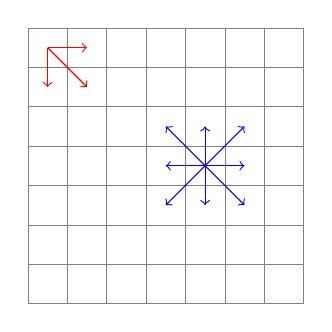
\begin{tikzpicture}[scale=.5]
  \draw[step=1cm,gray,very thin] (-3,-3) grid (4,4);
	\draw[->, red ] (-2.5,3.5) -- (-1.5, 3.5);
	\draw[->, red ] (-2.5,3.5) -- (-1.5, 2.5);
	\draw[->, red ] (-2.5,3.5) -- (-2.5, 2.5);
	\draw[->, blue] (1.5, 0.5) -- (0.5, 0.5);
	\draw[->, blue] (1.5, 0.5) -- (2.5, 0.5);
	\draw[->, blue] (1.5, 0.5) -- (1.5, 1.5);
	\draw[->, blue] (1.5, 0.5) -- (1.5,-0.5);
	\draw[->, blue] (1.5, 0.5) -- (0.5, 1.5);
	\draw[->, blue] (1.5, 0.5) -- (0.5,-0.5);
	\draw[->, blue] (1.5, 0.5) -- (2.5, 1.5);
	\draw[->, blue] (1.5, 0.5) -- (2.5,-0.5);
\end{tikzpicture}
\]
Then a generalized Moore machine of the form $S\yon^S\to p$, where
\[
p= \sum_{(i,j)\in\ord{n}\times\ord{n}}\yon^{d(i)\times d(j)},
\]
is one that has more movement options when it is in the center of the grid than when it is on the sides or corners.
\end{example}

\begin{exercise}
Add to \cref{ex.movement_options} as follows.
\begin{enumerate}
	\item Redefine $p$ so that at each grid value, the robot can receive not only the set of directions it can move in but also a reward value in $\rr$. 
	\item Define the set $S$ of robot states so that an element $s\in S$ includes both the robot's position and a list of all reward values so far.
	\item Define a morphism of polynomials $S\yon^S\to p$ in a way that respects positions and properly updates the robots list of rewards, but otherwise does anything you want.
\qedhere
\end{enumerate}
\end{exercise}

\begin{example}\label{ex.generalized_file_reader}
In \cref{exc.file_reader} one is tasked with making a file reader $\Sys{FileReader}$, where a file is a function $f\colon\ord{n}\to\Set{ascii}$. Now we take that same idea but make the robot have a different interface when it is in read-mode: namely, one where it cannot take in signals.

Let $State{FileReader} \coloneqq \{(s,t)\mid 1\leq s\leq t\leq n\}$ consist of a
current position $s$ and a terminal position $t$. For our interface, we'll have
two modes, each of which exposes an ascii character:
$$\Out{FileReader} = \langle \fun{Accepting}(c),\, \fun{Busy}(c) \mid c \in \Set{ascii} \rangle$$
%%
%% Jaz: In Haskell, this would read
%%      data \Out{FileReader} = Accepting ascii | Busy ascii
%%
For our input, we need a family $\In{FileReader} : \Out{FileReader} \to \smset$.
We'll define this by cases:
\begin{align*}
  \In{FileReader}(\fun{Accepting}(c)) &= \State{FileReader}, \\
  \In{FileReader}(\fun{Busy}(c)) &= \ord{1}.
\end{align*}

Our file reader will be $\fun{Accepting}$ if its current position is the
terminal position; otherwise, it will be $\fun{Busy}$. In either case, it will
expose the ascii character at the current position.
\begin{align*}
  \expose{FileReader}(s, t) = \begin{cases} \fun{Accepting}(f(s)) &\mbox{if $s = t$}\\ \fun{Busy}((f(s)))  \end{cases}
\end{align*}

While the file reader is $\fun{Busy}$, it will step forward through the file.
When it is $\fun{Accepting}$, it will set its new current and terminal position
to be the input. 
\begin{align*}
  \update{FileReader}(s, t) = \begin{cases} \_ \mapsto (s + 1, t) &\mbox{if $\expose{FileReader}(s, t)$ is $\fun{Busy}$} \\ (s', t') \mapsto (s', t') &\mbox{if $\expose{FileReader}(s, t)$ is $\fun{Accepting}$}  \end{cases}
\end{align*}

Let $A\coloneqq\{(s,t)\mid 1\leq s\leq t\leq n\}$, and let $p\coloneqq \Set{ascii}\mdot\yon^A+\Set{ascii}\mdot\yon^\1$; we construct a morphism in $\poly$
\[
(r_1,r^\sharp)\colon A\yon^A\to \Set{ascii}\mdot\yon^A+\Set{ascii}\mdot\yon^\1
\]
as follows.

$$A + B = \langle \fun{inl}(a), \fun{inr}(b) \mid a \in A, b \in B \rangle$$

$$A +_C B = \langle \fun{inl}(a), \fun{inr}(b) \mid a \in A, b \in B, \forall c
\in C.
\fun{inl}(f(c)) = \fun{inr}(g(c)) =\rangle$$


On positions define
\[
	r_1(s,t)\coloneqq
	\begin{cases}
		\const{inl}\ f(s)&\tn{ if } s=t\\
		\const{inr}\ f(s)&\tn{ if } s<t
	\end{cases}
\]

\[
	r^\sharp_{(t,t)}(s',t')\coloneqq (s',t')
	\qquad
	r^\sharp_{(s,t)}(1)\coloneqq (s+1,t)
\]
\end{example}

\begin{exercise}
Make a file reader that acts like that in \cref{ex.generalized_file_reader}, except that it only emits output $o\in\2\5\6$ when $o=100$.
\end{exercise}

%---- Subsection ----%
\subsection{Wiring diagrams}


%-------- Section --------%
\section{Bonus math about the category $\poly$}

\begin{exercise}
Show that the category $\poly$ has finite coproducts as follows.
\begin{enumerate}
	\item Show that $\0$ is an initial object in $\poly$, i.e.\ that for any polynomial $p$ there is a unique morphism $\0\to p$.
	\item Show that the standard sum of polynomials $p_1+p_2$ is a coproduct of $p_1$ and $p_2$. That is, provide morphisms $p_1\to p_1+p_2\from p_2$ and show that for any other $q$ with morphisms $p_1\To{f_1} q\From{f_2} p_2$, there exists a unique morphism $p_1+p_2\to q$---shown dashed---making the following diagram commute 
	\[
	\begin{tikzcd}
		p_1\ar[r]\ar[dr, "f_1"']&
		p_1+p_2\ar[d, dashed]&
		p_2\ar[l]\ar[dl, "f_2"]\\&
		q
	\end{tikzcd}
	\qedhere
	\]
\end{enumerate}
\end{exercise}


\begin{exercise}\label{exc.practice_sum_prod}
Let $p,q$ be polynomials as in \cref{prop.poly_maps_colax_prod_sum}. 
\begin{enumerate}
\item Is it true that the following are isomorphic?
\[
  \prod_{i\in p(\1)}\sum_{j\in q(\1)}{p_i}^{q_j}
  \cong^?
  \prod_{i\in p(\1)}\sum_{j\in q(\1)}\prod_{d\in q_j}\sum_{c\in p_i}\1
\]
\item Here's another way to think of maps in $\poly$; it'll be useful in \cref{exc.mono_epi_poly}. Show that there is an isomorphism
	\[
	\poly(p,q)\cong\sum_{f_1\colon p(\1)\to q(\1)}\prod_{j\in q(\1)}\smset\Big(q_j,\prod_{\{i\in p(\1)\mid i\mapsto j\}}p_i\Big).
	\]
	Say how any element of the right-hand side gives a way of delegating decisions from $p$ to $q$.
\end{enumerate}
\end{exercise}



\begin{exercise}\label{exc.mono_epi_poly}
Suppose $p,q\in\poly$ are polynomials and $f=(f_1,f^\sharp)\colon p\to q$ is a morphism with notation as in \cref{eqn.colax_poly_map}.
\begin{enumerate}
	\item Under what conditions is $f$ a monomorphism?
	\item Under what conditions is $f$ an epimorphism? Hint: use \cref{exc.practice_sum_prod}, \#2.
	\item Suppose $f$ is both a mono and an epi; it is an iso? (That is, is $\poly$ \emph{balanced}?)
	\item Can every morphism in $\poly$ be factored as an epic followed by a monic? Hint: use \cref{exc.practice_sum_prod}, \#2 again.
\qedhere
\end{enumerate}
\end{exercise}



%---- Subsection ----%
\subsection{Limits, colimits, and cartesian closure}

\begin{proposition}\label{prop.coprod_prod_poly}
The category $\poly$ has coproducts and products.
\end{proposition}
\begin{proof}
Let $A$ be a set and $p\colon A\to\poly$ a collection of polynomials $(p_a)_{a\in A}$.%
\footnote{
This is potentially ambiguous notation because $p_i$ generally denotes the exponent of the $i$th summand of polynomial $p$; we apologize for this. To be clear, to each $a\in A$ there is an associated polynomial $p_a\in\poly$. To write out $p_a$ as a sum of representables, we would say $p_a=\sum_{i\in p_a(\1)}\yon^{(p_a)_i}$.
}
Their coproduct is
\begin{equation}\label{eqn.sum_polys}
\sum_{a\in A}p_a=\sum_{a\in A}\sum_{i\in p_a(\1)}\yon^{(p_a)_i}\cong\sum_{(a,i)\in\sum_{a\in A}p_a(\1)}\yon^{(p_a)_i}
\end{equation}
which is manifestly a sum of representables, i.e.\ a polynomial, and which one can check satisfies the universal property of coproduct; see \cref{exc.check_coprod_prod}.

We claim that the product of this collection is
\begin{equation}\label{eqn.prod_polys}
\prod_{a\in A}p_a=
\prod_{a\in A}\sum_{i\in p_a(\1)}\yon^{(p_a)_i}\cong
\sum_{i\colon \prod_{a\in A}p_a(\1)}\yon^{\sum_{a\in A}p_{i(a)}}.
\end{equation}
Again, it is a sum of representables, so a polynomial, and one can check that it satisfies the universal property of product; see \cref{exc.check_coprod_prod}.
\end{proof}

\begin{exercise}\label{exc.check_coprod_prod}
Finish the proof of \cref{prop.coprod_prod_poly} as follows.
\begin{enumerate}
	\item Show that \eqref{eqn.sum_polys} satisfies the universal property for coproduct of polynomials.
	\item Show that \eqref{eqn.prod_polys} satisfies the universal property for product of polynomials.
\qedhere
\end{enumerate}
\end{exercise}

\begin{exercise}
Let $A=\2$ and $p\colon A\to\poly$ be given by $p_1\coloneqq\yon+\1$ and $p_2\coloneqq\yon+\2$. What is $\prod_{i\in\2}p_i$ according to \cref{eqn.prod_polys}? Does it check out?
\end{exercise}

\begin{proposition}
The category $\poly$ is completely distributive, i.e.\
\spiz{finish}
\end{proposition}

For any two polynomials $q,r$, define $r^q\in\poly$ by the following formula
\begin{equation}\label{eqn.exponential}
  r^q\coloneqq\prod_{i\in q(\1)}r\circ(\yon+q_j)
\end{equation}
where $\circ$ denotes composition.

Before proving that this really is an exponential in $\poly$, which we do in \cref{thm.poly_cart_closed}, we first get some practice with it.

\begin{example}
Let $A$ be a set. We've been writing the polynomial $A\yon^\0$ simply as $A$ and the polynomial $\yon^\1$ simply as $\yon$, so it better be true that the there is an isomorphism 
\[\yon^A\cong (\yon^\1)^{(A\yon^\0)}\]
in order for the notation to be consistent. Luckily, this is true. Checking \eqref{eqn.exponential}, we have
\[(\yon^\1)^{A\yon^\0}=\prod_{a\in A}\yon\circ(\0+\yon)\cong\yon^A\]
\end{example}

\begin{exercise}
Compute the following exponentials in $\poly$ using \eqref{eqn.exponential}:
\begin{enumerate}
	\item $p^\0$ for an arbitrary $p\in\poly$.
	\item $p^\1$ for an arbitrary $p\in\poly$.
	\item $\1^p$ for an arbitrary $p\in\poly$.
	\item $A^p$ for an arbitrary $p\in\poly$ and $A\in\smset$.
	\item $\yon^\yon$.
	\item $\yon^{\4\yon}$.
	\item $(\yon^A)^{\yon^B}$ for arbitrary sets $A,B\in\smset$.
\qedhere
\end{enumerate}
\end{exercise}


\begin{theorem}\label{thm.poly_cart_closed}
The category $\poly$ is Cartesian closed. That is, we have a natural isomorphism
\[
  \poly(p,r^q)\cong\poly(p\times q,r),
\]
where $r^q$ is the polynomial defined in \eqref{eqn.exponential}.
\end{theorem}
\begin{proof}
We have the following chain of natural isomorphisms
\begin{align*}
	\poly(p,r^q)&\cong
	\poly\Big(p,\prod_{j\in q(\1)}r\circ (\yon+q_j)\Big)\\&\cong
	\prod_{j\in q(\1)}\poly(p,r\circ(\yon+q_j))\\&\cong
	\prod_{j\in q(\1)}\prod_{i\in p(\1)}\poly(\yon^{p_i},r\circ(\yon+q_j))\\&\cong
	\prod_{i\in p(\1)}\prod_{j\in q(\1)}r\circ(p_i+q_j)\\&\cong
	\prod_{i\in p(\1)}\prod_{j\in q(\1)}\sum_{k\in r(\1)}(p_i+q_j)^{r_k}\\&\cong
	\poly(p\times q,r).
\end{align*}
The last step uses \cref{eqn.main_formula,prop.poly_times}.
\end{proof}


\begin{exercise}
Using \cref{eqn.exponential}, show that the functor $\smset\to\poly$ sends exponentials to exponentials.
\end{exercise}

\begin{theorem}\label{thm.poly_limits}
The category $\poly$ has all limits.
\end{theorem}
\begin{proof}
Recall that a category has all limits iff it has equalizers and products, so by \cref{prop.coprod_prod_poly} it suffices to show that $\poly$ has equalizers. 

Let $f_1,f_2\colon p\tto q$ be two maps of polynomials. Let $E\to p(\1)\tto q(\1)$ be an equalizer of the functions $f_1(\1),$ and $f_2(\1)$ in $\smset$. For each $e\in E$, write $f(e)\coloneqq f_1(e)=f_2(e)$; we have two polynomial morphisms $\yon^{p_e}\tto\yon_{q_{f(e)}}$, i.e.\ two functions $q_{f(e)}\tto p_e$. Defining $p'_e\in\smset$ to be their coequalizer, we can define a polynomial $p'$ as follows:
\[
  p'\coloneqq\sum_{e\in E}\yon^{p'_e}
\]
which comes equipped with a morphism $g\colon p'\to p$. One can check that it is an equalizer of $f_1,f_2$; see \cref{exc.poly_limits}.
\end{proof}

\begin{exercise}\label{exc.poly_limits}
Complete the proof of \cref{thm.poly_limits} as follows:
\begin{enumerate}
	\item We said that $p'$ comes equipped with a morphism $g\colon p'\to p$; what is it?
	\item Show that $g\then f_1=g\then f_2$.
	\item Show that $g$ is an equalizer of the pair $f_1,f_2$.
\qedhere
\end{enumerate}
\end{exercise}

\begin{exercise}
Let $p$ be any polynomial.
\begin{enumerate}
	\item There is a canonical choice of morphism $\eta\colon p\to p(\1)$; what is it?
	\item Suppose given an element $i\in p(\1)$, i.e.\ a function $\1\to p(\1)$.
	\item What is the pullback
	\[
	\begin{tikzcd}
	?\ar[r]\ar[d]&
	p\ar[d, "\eta"]\\
	\1\ar[r, "i"']&
	p(\1)\ar[ul, phantom, very near end, "\lrcorner"]
	\end{tikzcd}
	\qedhere
	\]
\end{enumerate}
\end{exercise}

Arbitrary colimits will be much less useful to us than limits, so the following theorem is included only for completeness; the reader can feel free to skip it.
\begin{theorem}\label{thm.poly_colimits}
The category $\poly$ has all colimits.
\end{theorem}
\begin{proof}
Recall that a category has all colimits iff it has coequalizers and coproducts, so by \cref{prop.coprod_prod_poly} it suffices to show that $\poly$ has coequalizers.

Let $f_1,f_2\colon p\tto q$ be two maps of polynomials. The pair of functions
\[f_1(\1),f_2(\1)\colon p(\1)\tto q(\1)\] 
define a graph $G\colon\fbox{$\bullet\tto\bullet$}\to\smset$ whose set $C$ of connected components is given by the coequalizer $g\colon q(\1)\to C$ of $f_1(\1)$ and $f_2(\1)$. The coequalizer of $f_1$ and $f_2$ will turn out to be a $C$-indexed sum of representables, each of which is given by a limit of a diagram of representables from $p$ and $q$, but expressing this limit, as we proceed to do, is a bit involved.

For each connected component $c\in C$, we have a connected subgraph $G_c\ss G$ with vertices $V_c\coloneqq g\inv(c)$ and edges $E_c\coloneqq f_1\inv(g\inv(c))=f_2\inv(g\inv(c))$. Note that $E_c\ss p(\1)$ and $V_c\ss q(\1)$, so to each $e\in E_c$ (resp.\ to each $v\in V_c$) we have an associated representable $\yon^{p_e}$ (resp.\ $\yon^{q_v}$).

The category of elements $\int G_c$ is a bipartite graph with objects $V+E$ and with two sorts of morphisms, $e\to f_1(e)$ and $e\to f_2(e)$, associated to each $e\in E_c$; all non-identity arrows point from an object in $E$ to an object in $V$. There is a functor $F\colon(\int G_c)\op\to\smset$ sending every $v\mapsto q_v$, every $e\mapsto p_e$, and every morphism to a function between them, namely either $(f_1^\sharp)_e\colon q_{f_1(e)}\to p_e$ or $(f_2^\sharp)_e\colon q_{f_2(e)}\to p_e$. Define $q'_c\in\smset$ to be the limit $q'_c\coloneqq\lim F\in\smset$ of $F$.

We claim that $q'\coloneqq\sum_{c\in C}\yon^{q'_c}$ is the coequalizer of $f_1$ and $f_2$. We leave the completion proof to the interested reader in \cref{exc.poly_colimits}.
\end{proof}

\begin{exercise}\label{exc.poly_colimits}
Complete the proof of \cref{thm.poly_colimits} as follows:
\begin{enumerate}
	\item Provide a map $g\colon q\to q'$ and show that $f_1\then g=f_2\then g$.
	\item Show that $g$ is a coequalizer of the pair $f_1,f_2$.
\qedhere
\end{enumerate}
\end{exercise}


%---- Subsection ----%
\subsection{Special polynomials and adjunctions}

There are a few special classes of polynomials that are worth discussing: 
\begin{enumerate}
	\item constant polynomials $\0,\1,\2,A$; 
	\item linear polynomials $\0,\yon, \2\yon, A\yon$;
	\item pure-powers polynomials, $\1, \yon, \yon^\2, \yon^A$; and 
	\item monomials $\0, A, \yon, \2\yon^\3, A\yon^B$.
\end{enumerate}
The first two classes, constant and linear, are interesting because they both put a copy of $\smset$ inside $\poly$, as we'll see in \cref{prop.ff_const_set_to_poly,prop.ff_lin_set_to_poly}. The third puts a copy of $\smset\op$ inside $\poly$, and the fourth puts a copy of something called ``bimorphic lenses'' inside $\poly$. We go through these four classes in order and then discuss some adjunctions that involve some of them.

\begin{proposition}\label{prop.ff_const_set_to_poly}
There is a fully faithful functor $\smset\to\poly$ sending $A\mapsto A\yon^\0=A$.
\end{proposition}
\begin{proof}
By \cref{eqn.colax_poly_map}, a map $f\colon A\yon^\0\to B\yon^\0$ consists of a function $f\colon A\to B$ and for each $a\in A$ a function $\0\to\0$. There is only one such function, so $f$ can be identified with just a map of sets $A\to B$.
\end{proof}

\begin{proposition}\label{prop.ff_lin_set_to_poly}
There is a fully faithful functor $\smset\to\poly$ sending $A\mapsto A\yon$.
\end{proposition}
\begin{proof}
By \cref{eqn.colax_poly_map}, a map $f\colon A\yon^\1\to B\yon^\1$ consists of a function $f\colon A\to B$ and for each $a\in A$ a function $\1\to\1$. There is only one such function, so $f$ can be identified with just a map of sets $A\to B$.
\end{proof}

\begin{theorem}\label{thm.adjoint_quadruple}
$\poly$ has an adjoint quadruple with $\smset$:
\begin{equation*}%\label{eqn.adjoints_galore}
\begin{tikzcd}[column sep=60pt]
  \smset
  	\ar[r, shift left=7pt, "A" description]
		\ar[r, shift left=-21pt, "A\yon"']&
  \poly
  	\ar[l, shift right=21pt, "p(\0)"']
  	\ar[l, shift right=-7pt, "p(\1)" description]
	\ar[l, phantom, "\scriptstyle\Leftarrow"]
	\ar[l, phantom, shift left=14pt, "\scriptstyle\Rightarrow"]
	\ar[l, phantom, shift right=14pt, "\scriptstyle\Rightarrow"]
\end{tikzcd}
\end{equation*}
where the functors have been labeled by where they send $A\in\smset$ and $p\in \poly$. 

Both rightward functors are fully faithful.
\end{theorem}
\begin{proof}
For any set $A$, there is a functor $\poly\to\smset$ given by sending $p$ to $p(A)$; it is $\poly(A,-)$. This, together with \cref{prop.ff_const_set_to_poly,prop.ff_lin_set_to_poly} give us the four functors and the fact that the two rightward functors are fully faithful. It remains to provide the following three natural isomorphisms:
\[
\smset(A,p(\0))\cong\poly(A,p)\qquad
\smset(p(\1),A)\cong\poly(p,A)\qquad
\smset(A,p(\1))\cong\poly(A\yon,p).
\]
All three come from our main formula, \cref{eqn.main_formula}; we leave the details to the reader in \cref{exc.adjoint_quadruple}.
\end{proof}

\begin{exercise}\label{exc.adjoint_quadruple}
Here we prove the remainder of \cref{thm.adjoint_quadruple} using \cref{eqn.main_formula}:
\begin{enumerate}
	\item Provide a natural isomorphism $\smset(A,p(\0))\cong\poly(A,p)$.
	\item Provide a natural isomorphism $\smset(p(\1),A)\cong\poly(p,A)$.
	\item Provide a natural isomorphism $\smset(A,p(\1))\cong\poly(A\yon,p)$.
\qedhere
\end{enumerate}
\end{exercise}

In \cref{thm.adjoint_quadruple} we see that $p\mapsto p(\0)$ and $p\mapsto p(\1)$ have left adjoints. This is true more generally for any set $A$ in place of $\0$ and $\1$, as we show in \cref{cor.substituting_adj}. However, the fact that $p\mapsto p(\1)$ is also a right adjoint---and hence that there is this \emph{quadruple} of adjunctions---is special to $A=\0,\1$.


\begin{proposition}\label{prop.two_var_adj}
There is a two-variable adjunction between $\smset$, $\poly$, and $\poly$:
\begin{align}\label{eqn.two_var_adj}
\poly(Ap,q)\cong\poly(p,q^A)\cong\smset(A,\poly(p,q)).
\end{align}
\end{proposition}
\begin{proof}
For any sets $A,B\in\smset$ and polynomial $q=\sum_{j\in q(\1)}\yon^{q_j}$, we need to check that there is a natural isomorphism
\[
\smset(A,q(B))\cong\poly(A\yon^B,q).
\]
This follows from our main formula \cref{eqn.main_formula}, since setting $p\coloneqq A\yon^B$ we have $p(\1)\cong A$ and $q(B)=\sum_{j\in q(\1)}B^{q_j}$.
\end{proof}

Using $p\coloneqq\yon^A$ and the Yoneda lemma, \cref{prop.two_var_adj} specializes to the following.


\begin{corollary}\label{cor.substituting_adj}
For any set $B$ there is an adjunction
\[
\adj{\smset}{A\yon^B}{p(B)}{\poly}
\]
where the functors are labeled by where they send $p\in\poly$ and $A\in\smset$.
\end{corollary}

\begin{exercise}
Prove \cref{cor.substituting_adj}.
\end{exercise}

\begin{proposition}
The Yoneda embedding $A\mapsto \yon^A$ has a left adjoint
\[
\adjr{\smset\op}{\yon^-}{\Gamma}{\poly}
\]
where $\Gamma(p)\coloneqq\prod_{i\in p(\1)}p_i$.
\end{proposition}
\begin{proof}
We have the following chain of natural isomorphisms:
\begin{align*}
  \smset(A,\Gamma(p))&\cong
  \Big(\prod_{i\in p(\1)}p_i\Big)^A
  	&\text{Definition of function}\\&\cong
  \prod_{i\in p(\1)}{p_i}^A
  	&\text{Definition of product}\\&\cong
  \prod_{i\in p(\1)}\sum_{j\in\1}{p_i}^A
  	&\text{Trivial sum}\\&\cong
  \poly(p,\yon^A).&\cref{eqn.main_formula}
\qedhere
\end{align*}

\end{proof}





%-------- Section --------%
\section{Dynamical systems}

%-------- Section --------%
\section{Wiring together dynamical systems}


















\end{document}
